\documentclass[review,3p,authoryear]{elsarticle}
% Target: Information Processing & Management (Elsevier). Switch to [final,5p,twocolumn] for a preview.
\usepackage[T1]{fontenc}
\usepackage[utf8]{inputenc}
\usepackage{amsmath,amssymb}
\usepackage{booktabs}
\usepackage{graphicx}
\usepackage{xcolor}
\usepackage{multirow}
\usepackage{makecell}
\usepackage{subcaption}
\usepackage[hidelinks]{hyperref}
\usepackage{lineno}
\usepackage{amsthm}
\theoremstyle{definition}
\newtheorem*{protocol}{Reporting protocol}
\theoremstyle{plain}
\newtheorem{proposition}{Proposition}
\graphicspath{{figures/}{../figures/}}
\setlength{\emergencystretch}{2em}
% generated by src/paper_numbers.py - do not edit by hand
\newcommand{\BAGap}{0.33}
\newcommand{\BARankShare}{84\%}
\newcommand{\BARecRank}{49\%}
\newcommand{\BBdedAUC}{0.823}
\newcommand{\BBdedFone}{59.15}
\newcommand{\BBexact}{850}
\newcommand{\BBfinal}{14{,}041}
\newcommand{\BBgroupAUC}{0.687}
\newcommand{\BBlosoAUC}{0.791}
\newcommand{\BBlosoMax}{0.911}
\newcommand{\BBlosoMin}{0.651}
\newcommand{\BBlosoN}{20}
\newcommand{\BBnPub}{19}
\newcommand{\BBrateMax}{66\%}
\newcommand{\BBrateMin}{7\%}
\newcommand{\BBraw}{15{,}056}
\newcommand{\BBrelAUC}{0.834}
\newcommand{\BBrelAcc}{77.72}
\newcommand{\BBrelFone}{64.37}
\newcommand{\BBrelSVMFone}{63.79}
\newcommand{\BBrelTCFone}{61.29}
\newcommand{\BBseedAUC}{0.821}
\newcommand{\BBseedAUCsd}{0.011}
\newcommand{\BBseedFone}{0.620}
\newcommand{\CellsBelowHalf}{19\%}
\newcommand{\DGEANN}{0.632}
\newcommand{\DGEANNDelta}{$-$0.028}
\newcommand{\DGEANNP}{=0.384}
\newcommand{\DGENDEF}{0.643}
\newcommand{\DGENDEFDelta}{$-$0.018}
\newcommand{\DGENDEFP}{=0.683}
\newcommand{\DGERMlr}{0.660}
\newcommand{\DGERMmlp}{0.639}
\newcommand{\DGERMmlpDelta}{$-$0.021}
\newcommand{\DGERMmlpP}{=0.384}
\newcommand{\DGMDFEND}{0.614}
\newcommand{\DGMDFENDDelta}{$-$0.046}
\newcommand{\DGMDFENDP}{=0.070}
\newcommand{\DGrecEM}{$-$221\%}
\newcommand{\DefPPRErr}{0.34}
\newcommand{\DupIW}{18}
\newcommand{\DupPT}{58}
\newcommand{\DupPTs}{128}
\newcommand{\ECEem}{0.476}
\newcommand{\ECEin}{0.046}
\newcommand{\ECEout}{0.328}
\newcommand{\EMgainPriorRho}{0.19}
\newcommand{\EMpriorErr}{0.46}
\newcommand{\ErrACC}{0.41}
\newcommand{\ErrEMvar}{0.46}
\newcommand{\ErrSrcPPR}{0.12}
\newcommand{\FTInAUC}{0.867}
\newcommand{\FTOffAUC}{0.559}
\newcommand{\FTOffFdef}{0.418}
\newcommand{\FTOffForc}{0.571}
\newcommand{\FTPairAUC}{0.614}
\newcommand{\FTRankShare}{59\%}
\newcommand{\FTRecEM}{$-$51\%}
\newcommand{\FTRecRank}{77\%}
\newcommand{\FTbetterCells}{23}
\newcommand{\FTminusLRin}{$-$0.025}
\newcommand{\FTminusLRoff}{+0.001}
\newcommand{\FTminusLRp}{0.98}
\newcommand{\FTseeds}{3}
\newcommand{\FTsubInAUC}{0.892}
\newcommand{\FTsubOffAUC}{0.558}
\newcommand{\FTsubOffFdef}{0.462}
\newcommand{\FTsubOffForc}{0.566}
\newcommand{\FTsubPairAUC}{0.601}
\newcommand{\GCconflict}{356}
\newcommand{\GCexact}{1{,}174}
\newcommand{\GapOther}{0.44}
\newcommand{\GapPair}{0.31}
\newcommand{\GloveInAUC}{0.864}
\newcommand{\GloveOffAUC}{0.564}
\newcommand{\GroupGC}{0.807}
\newcommand{\GroupLIAR}{0.664}
\newcommand{\GroupPF}{0.840}
\newcommand{\GroupPHEME}{0.644}
\newcommand{\INLPaccAfter}{0.25}
\newcommand{\INLPaccBefore}{0.87}
\newcommand{\ISOTfiv}{6{,}098}
\newcommand{\ISOTreuters}{20{,}768}
\newcommand{\ISOTreutersReal}{20{,}761}
\newcommand{\InAUC}{0.914}
\newcommand{\InAUCmax}{0.914}
\newcommand{\InAUCmin}{0.864}
\newcommand{\InFone}{0.854}
\newcommand{\LCsixfourGC}{0.610}
\newcommand{\LCsixfourISOT}{0.983}
\newcommand{\LCsixfourLIAR}{0.567}
\newcommand{\LCsixfourWEL}{0.894}
\newcommand{\LLMFdef}{0.364}
\newcommand{\LLMFhalf}{0.610}
\newcommand{\LLMForc}{0.638}
\newcommand{\LLMFpm}{0.622}
\newcommand{\LLMauc}{0.657}
\newcommand{\LLMaucMax}{0.730}
\newcommand{\LLMaucMin}{0.574}
\newcommand{\LLMbetterTargets}{7}
\newcommand{\LLMgainMax}{0.13}
\newcommand{\LLMgainMin}{0.06}
\newcommand{\LLMitems}{4{,}532}
\newcommand{\LLMminusLR}{+0.099}
\newcommand{\LLMminusLRp}{9.5e-7}
\newcommand{\LLMppr}{0\%}
\newcommand{\LLMrankShare}{41\%}
\newcommand{\LLMrecHalf}{90\%}
\newcommand{\LocoBal}{0.659}
\newcommand{\LocoBalDelta}{-0.001}
\newcommand{\LocoBalP}{=1.000}
\newcommand{\LocoBestSingle}{0.671}
\newcommand{\LocoCORAL}{0.621}
\newcommand{\LocoCORALDelta}{-0.038}
\newcommand{\LocoCORALP}{<0.001}
\newcommand{\LocoCeiling}{0.914}
\newcommand{\LocoDrop}{0.636}
\newcommand{\LocoDropDelta}{-0.023}
\newcommand{\LocoDropP}{=0.006}
\newcommand{\LocoINLP}{0.605}
\newcommand{\LocoINLPDelta}{-0.054}
\newcommand{\LocoINLPP}{=0.001}
\newcommand{\LocoMask}{0.661}
\newcommand{\LocoMaskDelta}{+0.001}
\newcommand{\LocoMaskP}{=1.000}
\newcommand{\LocoMeanSingle}{0.567}
\newcommand{\LocoPooled}{0.660}
\newcommand{\LocoSVD}{0.647}
\newcommand{\LocoSVDDelta}{-0.013}
\newcommand{\LocoSVDP}{=0.043}
\newcommand{\MaskISOTAllIn}{0.996}
\newcommand{\MaskISOTAllPair}{0.650}
\newcommand{\MaskISOTEntsIn}{0.996}
\newcommand{\MaskISOTEntsPair}{0.657}
\newcommand{\MaskISOTNoneIn}{0.998}
\newcommand{\MaskISOTNonePair}{0.679}
\newcommand{\MaskISOTSourceIn}{0.997}
\newcommand{\MaskISOTSourcePair}{0.681}
\newcommand{\MaskISOTTimeIn}{0.998}
\newcommand{\MaskISOTTimePair}{0.692}
\newcommand{\MaskWELAllIn}{0.964}
\newcommand{\MaskWELAllPair}{0.810}
\newcommand{\MaskWELEntsIn}{0.965}
\newcommand{\MaskWELEntsPair}{0.833}
\newcommand{\MaskWELNoneIn}{0.980}
\newcommand{\MaskWELNonePair}{0.808}
\newcommand{\MaskWELSourceIn}{0.979}
\newcommand{\MaskWELSourcePair}{0.815}
\newcommand{\MaskWELTimeIn}{0.977}
\newcommand{\MaskWELTimePair}{0.831}
\newcommand{\MatchedInAUC}{0.861}
\newcommand{\MatchedOffAUC}{0.556}
\newcommand{\McFracSig}{\textsc{glove-lr} 36\%, \textsc{nb-svm} 21\%, \textsc{roberta-lr} 17\%, \textsc{style-gb} 47\%, \textsc{tfidf-svm} 12\%}
\newcommand{\NcellsBelowHalf}{8}
\newcommand{\Ntotal}{144{,}550}
\newcommand{\OPDef}{0.439}
\newcommand{\OPEM}{0.358}
\newcommand{\OPGMM}{0.510}
\newcommand{\OPHalf}{0.539}
\newcommand{\OPOracle}{0.565}
\newcommand{\OPPrior}{0.547}
\newcommand{\OPRank}{0.541}
\newcommand{\OffAUC}{0.567}
\newcommand{\OffAUCmax}{0.567}
\newcommand{\OffAUCmin}{0.547}
\newcommand{\OffFone}{0.439}
\newcommand{\OffFoneOracle}{0.565}
\newcommand{\OpShareAll}{30\%}
\newcommand{\OpShareOther}{32\%}
\newcommand{\OpSharePair}{21\%}
\newcommand{\OracleCF}{0.537}
\newcommand{\OracleCFbias}{0.028}
\newcommand{\OracleCFbiasSmall}{0.056}
\newcommand{\PADiw}{1.45}
\newcommand{\PADmax}{1.98}
\newcommand{\PADmin}{1.28}
\newcommand{\PADrho}{-0.01}
\newcommand{\PADrhoCI}{[-0.61, 0.69]}
\newcommand{\PSaccRecZero}{$-$32\%}
\newcommand{\PSemRecMax}{$-$43\%}
\newcommand{\PSgainMax}{0.11}
\newcommand{\PSgainMin}{0.02}
\newcommand{\PSrankMinus}{0.477}
\newcommand{\PSrankPlus}{0.491}
\newcommand{\PSrankZero}{0.548}
\newcommand{\PSrecMinus}{58\%}
\newcommand{\PSrecPlus}{22\%}
\newcommand{\PSrecZero}{81\%}
\newcommand{\PStrueMinus}{0.536}
\newcommand{\PStruePlus}{0.541}
\newcommand{\PairAUC}{0.624}
\newcommand{\PairedInAUC}{0.892}
\newcommand{\PermAUC}{0.502}
\newcommand{\PermAUCsd}{0.067}
\newcommand{\PermInAUC}{0.514}
\newcommand{\PriorOther}{0.12}
\newcommand{\PriorPair}{0.05}
\newcommand{\PromiseGapOther}{0.44}
\newcommand{\PromiseGapPair}{0.31}
\newcommand{\PvIsotEmpty}{447}
\newcommand{\PvIsotExact}{5{,}795}
\newcommand{\PvIsotFurther}{270}
\newcommand{\PvIsotFurtherTitle}{267}
\newcommand{\PvIsotRel}{44{,}898}
\newcommand{\PvIsotWork}{38{,}833}
\newcommand{\PvWelAfter}{24{,}540}
\newcommand{\PvWelExact}{8{,}458}
\newcommand{\PvWelExtra}{10}
\newcommand{\PvWelIsotText}{38{,}656}
\newcommand{\PvWelIsotTitle}{480}
\newcommand{\PvWelMD}{73c9675a4b3d09f86a6933d0b8d7d908}
\newcommand{\PvWelOne}{37{,}106}
\newcommand{\PvWelRel}{72{,}134}
\newcommand{\PvWelWork}{24{,}530}
\newcommand{\PvWelZero}{35{,}028}
\newcommand{\RankOther}{0.30}
\newcommand{\RankPair}{0.24}
\newcommand{\RankShareAll}{70\%}
\newcommand{\RankShareCF}{76\%}
\newcommand{\RankShareCI}{[63\%, 79\%]}
\newcommand{\RankShareDropMax}{72\%}
\newcommand{\RankShareDropMin}{67\%}
\newcommand{\RankShareOther}{68\%}
\newcommand{\RankSharePair}{79\%}
\newcommand{\RankWorseShare}{10\%}
\newcommand{\RecACC}{$-$27\%}
\newcommand{\RecEM}{$-$64\%}
\newcommand{\RecEMCI}{[$-$154\%, $-$27\%]}
\newcommand{\RecEMMax}{$-$41\%}
\newcommand{\RecEMMin}{$-$87\%}
\newcommand{\RecGMM}{57\%}
\newcommand{\RecHalf}{80\%}
\newcommand{\RecPrior}{86\%}
\newcommand{\RecPriorCI}{[64\%, 96\%]}
\newcommand{\RecRank}{81\%}
\newcommand{\RecRankCF}{104\%}
\newcommand{\RecRankCI}{[56\%, 91\%]}
\newcommand{\RecRankMax}{81\%}
\newcommand{\RecRankMin}{66\%}
\newcommand{\RecSrcPPR}{76\%}
\newcommand{\RobBetterCells}{17}
\newcommand{\RobInAUC}{0.861}
\newcommand{\RobMinusLRoff}{$-$0.005}
\newcommand{\RobMinusLRp}{0.44}
\newcommand{\RobOffAUC}{0.544}
\newcommand{\RobOffAUCsd}{0.008}
\newcommand{\RobOffFdef}{0.452}
\newcommand{\RobOffForc}{0.549}
\newcommand{\SlackFone}{0.014}
\newcommand{\SlackFoneMax}{0.037}
\newcommand{\SrcPriorErr}{0.09}
\newcommand{\StyleISOT}{0.999}
\newcommand{\StyleInAUC}{0.745}
\newcommand{\StyleOffAUC}{0.535}
\newcommand{\StyleShare}{57\%}
\newcommand{\StyleWEL}{0.951}
\newcommand{\SubLRInAUC}{0.895}
\newcommand{\SubLROffAUC}{0.549}
\newcommand{\SubLROffAUCsd}{0.008}
\newcommand{\SubLROffFdef}{0.435}
\newcommand{\SubLROffForc}{0.560}
\newcommand{\ThrOther}{0.02}
\newcommand{\ThrPair}{0.02}
\newcommand{\TopKISOTIn}{0.999}
\newcommand{\TopKISOTInMax}{0.985}
\newcommand{\TopKISOTInThousand}{0.991}
\newcommand{\TopKISOTPair}{0.673}
\newcommand{\TopKISOTPairMax}{0.580}
\newcommand{\TopKISOTPairThousand}{0.597}
\newcommand{\TopKWELIn}{0.984}
\newcommand{\TopKWELInMax}{0.949}
\newcommand{\TopKWELInThousand}{0.962}
\newcommand{\TopKWELPair}{0.827}
\newcommand{\TopKWELPairMax}{0.718}
\newcommand{\TopKWELPairThousand}{0.754}
\newcommand{\TopicGCBalIn}{0.799}
\newcommand{\TopicGCBalOut}{0.519}
\newcommand{\TopicGCDropped}{61\%}
\newcommand{\TopicGCPurity}{0.76}
\newcommand{\TopicGCRandIn}{0.846}
\newcommand{\TopicGCRandOut}{0.542}
\newcommand{\TopicISOTBalIn}{0.999}
\newcommand{\TopicISOTBalOut}{0.606}
\newcommand{\TopicISOTDropped}{65\%}
\newcommand{\TopicISOTPurity}{0.82}
\newcommand{\TopicISOTRandIn}{0.998}
\newcommand{\TopicISOTRandOut}{0.604}
\newcommand{\TopicLIARBalIn}{0.687}
\newcommand{\TopicLIARBalOut}{0.532}
\newcommand{\TopicLIARDropped}{21\%}
\newcommand{\TopicLIARPurity}{0.63}
\newcommand{\TopicLIARRandIn}{0.692}
\newcommand{\TopicLIARRandOut}{0.530}
\newcommand{\TopicWELBalIn}{0.986}
\newcommand{\TopicWELBalOut}{0.622}
\newcommand{\TopicWELDropped}{50\%}
\newcommand{\TopicWELPurity}{0.81}
\newcommand{\TopicWELRandIn}{0.984}
\newcommand{\TopicWELRandOut}{0.622}
\newcommand{\TwShared}{169}
\newcommand{\WELfiv}{125}
\newcommand{\WELnear}{815}
\newcommand{\WELnyt}{6{,}223}
\newcommand{\WELrelFiv}{6{,}261}
\newcommand{\WELrelNyt}{6{,}223}
\newcommand{\WELrelReu}{21{,}270}
\newcommand{\WELrelReuN}{21{,}289}
\newcommand{\XlBBEN}{0.777}
\newcommand{\XlBBtoEN}{0.931}
\newcommand{\XlBN}{0.813}
\newcommand{\XlEN}{0.994}
\newcommand{\XlENtoBB}{0.707}
\newcommand{\XlTransCost}{0.04}
\newcommand{\pairGCPFAUC}{0.59}
\newcommand{\pairGCPFCI}{[0.50, 0.68]}
\newcommand{\pairGCPFFdef}{0.425}
\newcommand{\pairGCPFForc}{0.595}
\newcommand{\pairGCPFFpm}{0.576}
\newcommand{\pairGCPFIn}{0.869}
\newcommand{\pairGCPFPPR}{0.07}
\newcommand{\pairGCPFPrior}{0.43}
\newcommand{\pairISOTWELFakeAUC}{0.69}
\newcommand{\pairISOTWELFakeCI}{[0.66, 0.71]}
\newcommand{\pairISOTWELFakeFdef}{0.539}
\newcommand{\pairISOTWELFakeForc}{0.638}
\newcommand{\pairISOTWELFakeFpm}{0.635}
\newcommand{\pairISOTWELFakeIn}{0.999}
\newcommand{\pairISOTWELFakePPR}{0.78}
\newcommand{\pairISOTWELFakePrior}{0.43}
\newcommand{\pairLIARPFAUC}{0.51}
\newcommand{\pairLIARPFCI}{[0.42, 0.60]}
\newcommand{\pairLIARPFFdef}{0.495}
\newcommand{\pairLIARPFForc}{0.536}
\newcommand{\pairLIARPFFpm}{0.517}
\newcommand{\pairLIARPFIn}{0.698}
\newcommand{\pairLIARPFPPR}{0.54}
\newcommand{\pairLIARPFPrior}{0.44}
\newcommand{\pairPFGCAUC}{0.53}
\newcommand{\pairPFGCCI}{[0.48, 0.56]}
\newcommand{\pairPFGCFdef}{0.464}
\newcommand{\pairPFGCForc}{0.517}
\newcommand{\pairPFGCFpm}{0.514}
\newcommand{\pairPFGCIn}{0.893}
\newcommand{\pairPFGCPPR}{0.54}
\newcommand{\pairPFGCPrior}{0.23}
\newcommand{\pairPFLIARAUC}{0.50}
\newcommand{\pairPFLIARCI}{[0.47, 0.54]}
\newcommand{\pairPFLIARFdef}{0.497}
\newcommand{\pairPFLIARForc}{0.509}
\newcommand{\pairPFLIARFpm}{0.502}
\newcommand{\pairPFLIARIn}{0.893}
\newcommand{\pairPFLIARPPR}{0.40}
\newcommand{\pairPFLIARPrior}{0.44}
\newcommand{\pairTwATwBAUC}{0.67}
\newcommand{\pairTwATwBCI}{[0.52, 0.82]}
\newcommand{\pairTwATwBFdef}{0.572}
\newcommand{\pairTwATwBForc}{0.646}
\newcommand{\pairTwATwBFpm}{0.597}
\newcommand{\pairTwATwBIn}{0.981}
\newcommand{\pairTwATwBPPR}{0.62}
\newcommand{\pairTwATwBPrior}{0.46}
\newcommand{\pairTwBTwAAUC}{0.66}
\newcommand{\pairTwBTwACI}{[0.55, 0.75]}
\newcommand{\pairTwBTwAFdef}{0.580}
\newcommand{\pairTwBTwAForc}{0.631}
\newcommand{\pairTwBTwAFpm}{0.591}
\newcommand{\pairTwBTwAIn}{0.967}
\newcommand{\pairTwBTwAPPR}{0.63}
\newcommand{\pairTwBTwAPrior}{0.51}
\newcommand{\pairWELFakeISOTAUC}{0.85}
\newcommand{\pairWELFakeISOTCI}{[0.82, 0.87]}
\newcommand{\pairWELFakeISOTFdef}{0.753}
\newcommand{\pairWELFakeISOTForc}{0.765}
\newcommand{\pairWELFakeISOTFpm}{0.763}
\newcommand{\pairWELFakeISOTIn}{0.989}
\newcommand{\pairWELFakeISOTPPR}{0.36}
\newcommand{\pairWELFakeISOTPrior}{0.46}

\journal{Information Processing \& Management}

\begin{document}
\begin{frontmatter}

\title{Mostly ranking, partly threshold: decomposing and repairing the cross-corpus generalisation gap of misinformation detectors}

\author[mu]{Dewan Fahad Chowdhury\corref{cor}\fnref{eq}}
\ead{dewanfahadc@gmail.com}
\author[mu]{Md.\ Rejaul Korim Sadi\fnref{eq}}
\cortext[cor]{Corresponding author.}
\fntext[eq]{These authors contributed equally to this work and share first authorship.}
\affiliation[mu]{organization={Department of Computer Science and Engineering, Metropolitan University},
            city={Sylhet},
            country={Bangladesh}}

\begin{abstract}
Fake-news detectors score near-perfectly on their training corpus and much worse elsewhere, but cross-domain studies report this with accuracy or F1, which conflates two failures with different remedies: ranking new items badly, and ranking them well but thresholding them wrongly. We separate the two. Ten public corpora in English and Bengali (articles, headlines, claims, tweets) are audited for label direction and near-duplicates, and six detectors are evaluated train-on-one, test-on-all with five seeds, bootstrap intervals and permutation controls. The audit finds that the two most used article corpora code labels in opposite directions, which turns moderate transfer into an apparent below-chance collapse, as well as label-conflicting duplicates and tweets shared across rumour corpora. Mean ROC-AUC falls from \InAUC{} in-domain to \OffAUC{} across corpora. Decomposing the lost macro-F1 attributes \RankShareAll{} to a ranking deficit and \OpShareAll{} to the operating point. The standard label-shift correction, EM prior adaptation, enlarges the operating-point loss because calibration does not transfer (expected calibration error \ECEin{} in-domain, \ECEout{} across corpora), whereas flagging the source's base rate of target items recovers \RecRank{} of it without target labels. Twenty-two surface statistics, publisher identity or 64 training examples recover much of the in-domain signal, and frozen RoBERTa features transfer no better than TF-IDF. Pooling six training corpora raises held-out AUC from \LocoMeanSingle{} to \LocoPooled{}, while removing corpus identity from the representation lowers it, because corpus and label are entangled. Bengali clickbait detection, in contrast, survives unseen publishers and languages. We release code, per-item scores and a reporting protocol.
\end{abstract}


\begin{highlights}
\item Ten audited corpora, six detectors, five seeds: train on one, test on all.
\item Most of the cross-corpus F1 gap is lost ranking; the rest is a mis-set threshold.
\item EM label-shift correction worsens the threshold: calibration does not transfer.
\item Flagging the source base rate of new items recovers most threshold loss, label-free.
\item Bengali clickbait transfers across publishers and languages; veracity does not.

\end{highlights}

\begin{keyword}
misinformation detection \sep fake news \sep cross-corpus generalisation \sep dataset audit \sep label shift \sep shortcut learning \sep Bengali
\end{keyword}
\end{frontmatter}

\linenumbers
\section{Introduction}\label{sec:intro}
False stories travel farther and faster than true ones on social platforms \citep{vosoughi2018spread}, and the cost of that asymmetry is borne by public health, elections and trust in institutions \citep{lazer2018science}. Automatic detection is one response, and on the standard benchmarks it appears close to solved: content-based classifiers routinely report accuracies above 95\% \citep{shu2017survey,zhou2020survey,kaliyar2021fakebert}. A detector, however, is deployed on data it was not trained on, and a growing body of work shows that these scores do not survive a change of corpus \citep{perezrosas2018automatic,janicka2019crossdomain,suprem2022generalizability,delloglio2026comparison} and that some of them reflect dataset artefacts rather than veracity \citep{asr2019bigdata,thibault2025guide,verma2026audit}.

What is still missing is an account of \emph{why} the transfer gap arises in a form that tells a practitioner what to do about it. A detector can fail on a new corpus in two different ways. It can \emph{order} the new items badly, scoring fabricated stories no higher than genuine ones; or it can order them well but place its decision threshold in the wrong place, because the new corpus has a different base rate or because its scores are scaled differently. The first failure needs a better representation; the second only needs a better operating point. Accuracy and F1, the metrics almost every cross-domain study reports, conflate the two.

This paper separates them. We assemble ten public corpora in two languages that cover four text units (articles, headlines, claims and tweets) and three constructs (veracity, rumour and clickbait), audit them for label direction and for within- and cross-corpus duplication, and evaluate six detectors in a train-on-one, test-on-all design with five seeds, bootstrap confidence intervals and permutation controls. We then decompose the macro-F1 that a detector loses on a new corpus into a ranking deficit, which no threshold can recover, and operating-point losses, which the right threshold would, and we evaluate label-free repairs aimed at each part. Our contributions are:

\begin{enumerate}
\item \textbf{An audited multi-corpus benchmark.} The two most used article corpora code their labels in opposite directions (ISOT: $1=$ fake; WELFake: $1=$ real). We show that simple signature probes detect such an inversion, which otherwise masquerades as a below-chance collapse of transfer, as it did in our own first pipeline. MinHash deduplication finds label-conflicting duplicates in GossipCop and source tweets shared between PHEME and Twitter15/16 (Section~\ref{sec:data}).
\item \textbf{A transfer gap decomposition.} Across 42 directed corpus pairs, \RankShareAll{} of the macro-F1 gap is a ranking deficit and \OpShareAll{} an operating-point loss (Section~\ref{sec:where}). Mean transfer AUC is \OffAUC{} against \InAUC{} in-domain; the gap is real but is not the collapse to chance that F1 alone suggests.
\item \textbf{A label-free operating-point repair, and why the standard one fails.} Expectation--maximisation prior adaptation, the textbook remedy for label shift, enlarges the operating-point loss (\RecEM{} recovered), because calibration does not survive the change of corpus. Transferring the ranking rule instead (flagging the source's base rate of target items) recovers \RecRank{} without any target label (Section~\ref{sec:op}).
\item \textbf{Evidence on what the detectors learn.} A model of 22 surface statistics and group identity alone recover much of the in-domain signal, 64 examples suffice on the article and tweet corpora, and the strongest cues are outlet signatures and time expressions; masking, feature deletion and topic balancing show how much of the ranking survives without them (Section~\ref{sec:shortcuts}). For the ranking deficit, training on several corpora at once raises held-out AUC from \LocoMeanSingle{} to \LocoPooled{}, whereas making the representation invariant to corpus identity (feature deletion, CORAL, nullspace projection) lowers it, because corpus identity and label are entangled in these benchmarks (Section~\ref{sec:repair-res}).
\item \textbf{A low-resource extension.} In Bengali, clickbait detection replicates the published baseline, survives held-out publishers and transfers across languages by translation, which suggests that whether a cue transfers depends on whether it \emph{is} the construct or merely correlates with it (Section~\ref{sec:bangla}).
\item \textbf{A reporting protocol and a full release} of code, seeds, per-cell results and predictions (Section~\ref{sec:discussion}).
\end{enumerate}

\section{Related work}\label{sec:related}

\paragraph{Cross-domain failure of fake-news detectors}
That content-based detectors degrade across domains has been reported since the first multi-domain corpora: models trained on one news domain lose much of their accuracy on another \citep{perezrosas2018automatic,janicka2019crossdomain}, cross-domain training needs domain-aware architectures \citep{silva2021crossdomain}, and fine-tuning on one COVID-19 corpus often hurts performance on related ones \citep{suprem2022generalizability}. \citet{bozarth2020evaluation} showed that conclusions about which model is best depend on the dataset, the evaluation type and the metric. Most recently, \citet{delloglio2026comparison} benchmarked twelve approaches on ten English corpora and found cross-dataset median F1 close to 0.5 for classical and fine-tuned models, with zero-shot large language models more stable, and \citet{hoy2025features} found stylistic and ``social-monetisation'' features to transfer better than token representations. These studies establish \emph{that} detectors fail to transfer, almost always through a single threshold-dependent score (accuracy or F1). They do not separate a loss of discrimination from a mis-set decision threshold, which is the distinction this paper is built on.

\paragraph{Shortcuts and dataset artefacts}
Shortcut learning, where a model exploits a spurious cue that predicts the label in the training distribution only, is a general failure mode of deep and shallow models alike \citep{geirhos2020shortcut,gururangan2018artifacts,mccoy2019right}. For misinformation, \citet{horne2017thisjustin} and \citet{schuster2020stylometry} showed how much of the signal is style rather than veracity, and \citet{asr2019bigdata} documented topical imbalance across fake-news corpora. \citet{verma2026audit} audited the ISOT corpus in depth: subject metadata alone separates the classes perfectly, a newswire tag marks 99.2\% of real articles, duplicates contaminate 19.4\% of a naive test split, deleting the 1{,}000 highest-weight unigrams leaves F1 at 0.926, and ISOT-trained models reach only near-chance ranking on LIAR. \citet{thibault2025guide} surveyed 75 misinformation datasets and found keyword--label correlations and temporal leakage in several of them, including Twitter15/16, ISOT and BanFakeNews. We build directly on these audits but differ in scope and in aim: we audit ten corpora jointly, including cross-corpus duplication and label direction, and we use the audit to explain and repair the transfer gap rather than only to document it.

\paragraph{Rumour benchmarks}
Rumour-detection benchmarks share the problem. On Twitter15/16 and PHEME, event-level spurious correlations inflate scores \citep{wu2022spurious}, chronological splits lower them \citep{mu2023time}, and simple text baselines rival propagation-based models \citep{pelrine2021simple}. We therefore treat the source posts of these corpora as one more text unit in our matrix and do not re-evaluate propagation models, which these works already cover.

\paragraph{Label shift and invariant representations}
Two families of methods from the domain-adaptation literature map onto the two parts of our decomposition. Label-shift adaptation re-estimates the target class prior from unlabelled predictions and adjusts the posteriors \citep{saerens2002adjusting,lipton2018bbse}; with calibrated scores, this simple expectation--maximisation procedure is hard to beat \citep{alexandari2020labelshift}. Representation methods instead try to remove domain information: correlation alignment matches feature covariances \citep{sun2016coral}, adversarial training removes domain-predictive directions \citep{ganin2016dann}, and iterative nullspace projection deletes linearly decodable attributes \citep{ravfogel2020inlp}. Domain-adaptation theory bounds target error by source error plus a domain divergence that can be estimated with a domain classifier \citep{bendavid2010theory}. In misinformation, label shift has been addressed mainly with pseudo-label correction inside neural adaptation pipelines; we are not aware of work that measures how much of the cross-corpus gap is a prior/threshold effect and how much a representation effect, and repairs each with the matching tool.

\paragraph{Large language models}
Zero-shot and few-shot large language models are less exposed to dataset-specific shortcuts because they are not trained on the benchmark \citep{pelrine2023gpt4,thibault2025guide,delloglio2026comparison}, and they can serve as advisers to smaller detectors \citep{hu2024badactor}. Supervised detectors nonetheless remain the cheapest and most widely deployed option, and the decomposition we propose applies to any detector that outputs a score, including a prompted language model.

\paragraph{Position of this work}
Table~\ref{tab:positioning} contrasts our study with the closest prior audits. The combination we contribute is a two-way, multi-corpus, multi-unit and bilingual matrix; a decomposition that attributes the gap to ranking or to the operating point; label-free repairs targeted at each part; and audit findings (label inversion, cross-corpus duplication) that change measured transfer.

\begin{table}[t]
\centering
\caption{Position relative to the closest prior audits: S\&P = \citet{suprem2022generalizability}; T = \citet{thibault2025guide}; V = \citet{verma2026audit}; D = \citet{delloglio2026comparison} ({\checkmark} present, -- absent; units: a = article, h = headline, c = claim, t = tweet).}\label{tab:positioning}
\footnotesize
\begin{tabular}{@{}p{5.2cm}ccccc@{}}
\toprule
 & S\&P & T & V & D & \textbf{This work} \\
\midrule
Corpora (languages) & 9 (en) & 75 (survey) & 2 (en) & 10 (en) & 10 (en, bn) \\
Text units & mixed & mixed & a, c & mixed & a, h, c, t \\
Full train$\times$test transfer matrix & {\checkmark} & -- & -- & {\checkmark} & {\checkmark} \\
Within- and cross-corpus near-duplicate control & -- & partial & {\checkmark} & -- & {\checkmark} \\
Label-direction verification & -- & -- & -- & -- & {\checkmark} \\
Threshold-free metrics (AUC, AP) & -- & -- & {\checkmark} & -- & {\checkmark} \\
Ranking vs.\ operating-point decomposition & -- & -- & partial & -- & {\checkmark} \\
Seeds, bootstrap CIs, permutation control & -- & -- & {\checkmark} & tests only & {\checkmark} \\
Label-free repair evaluated & reject opt. & -- & -- & MERMAID & EM, rank, INLP, CORAL \\
Low-resource language & -- & -- & -- & -- & Bengali \\
\bottomrule
\end{tabular}
\end{table}

\section{Corpora and data audit}\label{sec:data}

\subsection{Corpora}
We use ten public corpora (Table~\ref{tab:corpora}). Seven share the veracity construct and form the main transfer matrix: two article corpora, ISOT \citep{ahmed2017isot,ahmed2018isot} and WELFake \citep{verma2021welfake}; two headline corpora from FakeNewsNet, PolitiFact and GossipCop \citep{shu2020fakenewsnet}, for which the public release contains titles and URLs; the claim corpus LIAR \citep{wang2017liar}, obtained through LIAR-PLUS \citep{alhindi2018liarplus}, binarised as \{pants-fire, false\} versus \{mostly-true, true\} with the two middle grades dropped; and the source tweets of Twitter15 and Twitter16 \citep{ma2017kernel}, using their false and true classes. Three further corpora extend the analysis to other constructs and to Bengali: the source tweets of PHEME rumour/non-rumour threads \citep{zubiaga2016phemernr,zubiaga2017context}; an English clickbait headline corpus \citep{chakraborty2016clickbait}; and BanglaBait \citep{mahtab2023banglabait}, \BBraw{} labelled Bengali news articles with machine-translated English titles. Labels differ in what they assert: LIAR rates individual claims, FakeNewsNet and Twitter15/16 rate a story through a fact-check, and ISOT and WELFake label articles largely by the outlet they came from. We keep these distinctions explicit and draw the strongest conclusions from four \emph{same-task pairs} that hold unit and construct fixed: ISOT$\leftrightarrow$WELFake (articles), PolitiFact$\leftrightarrow$GossipCop (headlines, politics vs.\ entertainment), Twitter15$\leftrightarrow$Twitter16 (tweets, two collection windows), and LIAR$\leftrightarrow$PolitiFact (claims vs.\ headlines from the same fact-checker). Every label is mapped to $1=$ fake, false, rumour or clickbait.

\paragraph{Provenance of the article files}
For the two article corpora we start from cleaned working copies made at an earlier stage of this project, and we reconstructed both from the original releases to document exactly how they were made (the script is in the repository). The ISOT release has \PvIsotRel{} articles in two files, one per class. Our copy keeps \PvIsotWork{} of them, all with their release labels: it lacks \PvIsotExact{} exact title-and-text duplicates and \PvIsotFurther{} further articles, \PvIsotFurtherTitle{} of which repeat the title of an article that was kept. The \PvIsotEmpty{} articles with an empty body keep their headline and are scored on it. The WELFake release (Zenodo, MD5 \texttt{\PvWelMD}) has \PvWelRel{} articles merged from four earlier collections, one of them a Reuters-based news set like ISOT's real class \citep{verma2021welfake,welfake2021data}. Our copy keeps \PvWelWork{}. Removing \PvWelExact{} exact duplicates, the \PvWelIsotText{} articles whose text also appears in the ISOT release and \PvWelIsotTitle{} more whose title does reproduces it up to \PvWelExtra{} articles, and no article of our copy lies outside this reconstruction. The overlap step matters: without it, about three in five deduplicated WELFake articles would be ISOT articles, and ISOT$\leftrightarrow$WELFake transfer would be inflated. After it, only \DupIW{} near-duplicates of ISOT remain, and those are excluded from every test (Section~\ref{sec:audit}). The repository includes loaders for both releases, so the whole pipeline, including this cleaning, can be rerun from the public files.

\begin{table}[t]
\centering
\caption{Corpora after harmonisation and deduplication. ``Exact'' and ``near'' count removed duplicates; ``conflict'' counts items removed because duplicates disagreed on the label; ``pos.'' is the share labelled fake, false, rumour or clickbait. For LIAR and Twitter15/16, ``raw'' counts the items in the binary view (LIAR: pants-fire/false vs.\ mostly-true/true; Twitter: false vs.\ true).}\label{tab:corpora}
\small
\begin{tabular}{@{}llllrrrrrr@{}}
\toprule
Corpus & Unit & Construct & Lang. & Raw & Exact & Near & Conflict & Final & Pos. \\
\midrule
ISOT & article & veracity & en & 38{,}833 & 0 & 79 & 0 & 38{,}749 & 0.46 \\
WELFake & article & veracity & en & 24{,}530 & 0 & 815 & 6 & 23{,}708 & 0.43 \\
PolitiFact & headline & veracity & en & 1{,}056 & 71 & 3 & 6 & 976 & 0.43 \\
GossipCop & headline & veracity & en & 22{,}140 & 1{,}174 & 26 & 380 & 20{,}560 & 0.23 \\
LIAR & claim & veracity & en & 8{,}090 & 21 & 11 & 3 & 8{,}055 & 0.44 \\
Twitter15 & tweet & veracity & en & 742 & 55 & 14 & 0 & 673 & 0.51 \\
Twitter16 & tweet & veracity & en & 412 & 51 & 3 & 0 & 358 & 0.46 \\
\midrule
PHEME & tweet & rumour & en & 5{,}802 & 124 & 98 & 25 & 5{,}555 & 0.34 \\
ClickbaitEN & headline & clickbait & en & 32{,}000 & 2 & 123 & 0 & 31{,}875 & 0.50 \\
BanglaBait & headline & clickbait & bn & 15{,}056 & 850 & 124 & 41 & 14{,}041 & 0.34 \\
\bottomrule
\end{tabular}
\end{table}


\subsection{Audit}\label{sec:audit}
\paragraph{Label direction}
Corpora disagree on which value denotes ``fake'', and nothing in a CSV file says which convention it follows. We therefore verify label direction with \emph{signature probes}: strings that only a reliable or only a fabricating outlet produces. Figure~\ref{fig:audit}a shows the result for the two article corpora. In ISOT, \ISOTreutersReal{} of the \ISOTreuters{} ``(Reuters)'' datelines carry label~0 and all \ISOTfiv{} texts with the fake-site template ``Featured image via'' carry label~1, so $1=$ fake. WELFake is more treacherous, because its documentation and its file disagree. The release record gives the legend $0=$ fake, $1=$ real \citep{welfake2021data}, but the file uses the opposite coding: all \WELrelNyt{} titles ending in ``- The New York Times'' carry label~0, all \WELrelFiv{} texts with ``Featured image via'' carry label~1, and \WELrelReu{} of the \WELrelReuN{} ``(Reuters)'' datelines carry label~0. The class sizes say the same. Label~1 holds \PvWelOne{} articles and label~0 \PvWelZero{}, which are the numbers of fake and real articles stated in the same record. Our working copy was made by following the legend: every label is the inverse of the release label, and a class-name column calls the inverted label~1 ``fake''. Our first pipeline trusted that column. Read that way, every ISOT$\leftrightarrow$WELFake score is inverted and ISOT$\to$WELFake looks like a below-chance collapse, while in-domain accuracy and macro-F1 are unaffected, which is why the error is easy to miss. The probes exposed it, and the loader now reverses the labels of the copy (or reads the release with the coding its file actually uses). A ranking metric below 0.5 on a same-task pair should be treated as a symptom to investigate before it is reported as a finding.

\begin{figure}[t]
\centering
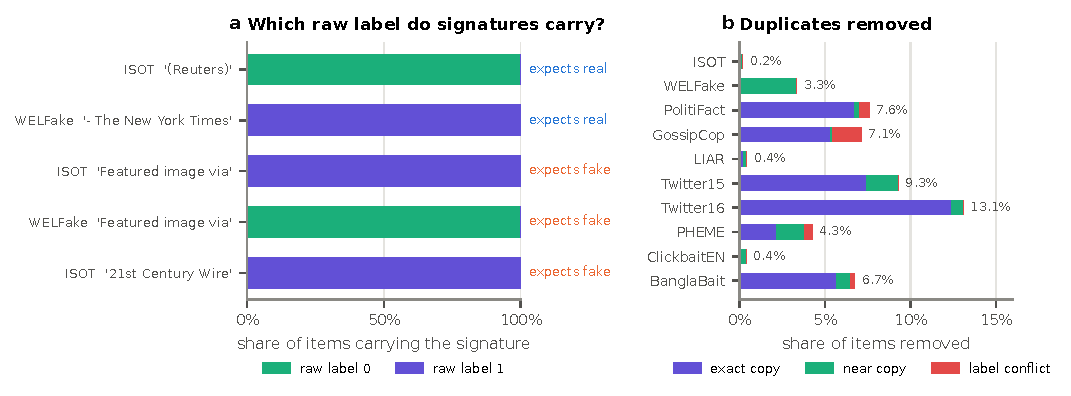
\includegraphics[width=\linewidth]{fig_audit}
\caption{Data audit. (a)~Label-direction probes: share of the items carrying an outlet signature that sit under raw label~0 or~1 (signatures found in at least 100 items). A reliable-outlet signature should sit under ``real'' and a fake-site signature under ``fake''. ISOT and the WELFake release both code $1=$ fake, although the WELFake record documents $0=$ fake; our working copy of WELFake, made by following that legend, has every label inverted. (b)~Share of items removed by deduplication: exact copies, near copies (MinHash, Jaccard $\geq0.8$) and items whose duplicates carried both labels.}\label{fig:audit}
\end{figure}

\paragraph{Duplicates}
Within each corpus we removed exact duplicates of the normalised text and then near-duplicates found by MinHash locality-sensitive hashing \citep{broder1997minhash} (128 permutations, Jaccard $\geq0.8$; word 3-grams for articles, character 5-grams otherwise). Groups whose members disagree on the label were dropped entirely. Table~\ref{tab:corpora} and Figure~\ref{fig:audit}b report the counts. Two corpora stand out. GossipCop contains \GCexact{} redundant exact copies of headlines, and a further \GCconflict{} rows whose headline appears under \emph{both} labels; BanglaBait contains \BBexact{} redundant exact copies of titles and, after deduplication, \BBfinal{} items. Even the cleaned WELFake copy still contained \WELnear{} near-duplicates.

\paragraph{Cross-corpus overlap}
Near-duplicates across corpora inflate transfer. ISOT and WELFake share only \DupIW{} near-duplicate articles, so the removal of shared articles from the WELFake copy worked. PHEME, however, shares \DupPT{} source tweets with Twitter15 and \DupPTs{} with Twitter16, because the corpora were collected around overlapping breaking-news events; Twitter15 and Twitter16 share \TwShared{} tweet identifiers, all labelled \emph{unverified}. Every transfer test excludes target items that are near-duplicates of the source corpus.

\section{Methodology}\label{sec:method}

\subsection{Evaluation protocol}\label{sec:protocol}
For every corpus and every seed $s\in\{0,\dots,4\}$ we draw a stratified 70/10/20 train/validation/test split. The seed also fixes model initialisation and any subsampling. Training splits are capped at 8{,}000 items, validation at 1{,}500 and test at 3{,}000 (stratified) so that the largest corpora do not dominate run time, and every cap is applied in the same way to every model. Featurisers (vocabularies, IDF weights, SVD bases) are fitted on the source training split only. Hyperparameters (the inverse regularisation strength $C\in\{0.25,1,4\}$, the number of boosting rounds, or the fine-tuning epoch) are selected on the source validation split by ROC-AUC. The selected model's scores are then Platt-calibrated \citep{platt1999probabilistic} on the same validation split, which makes the default operating point $t=0.5$ the Bayes decision under the source prior. No hyperparameter, threshold or calibration step sees a target label. When a model trained on corpus $A$ is tested on corpus $B$, test items of $B$ that are near-duplicates of any item of $A$ (Section~\ref{sec:audit}) are removed.

Three training regimes are run for every model except the fine-tuned transformer. \emph{Full} uses the capped training split. \emph{Matched} subsamples every source to $n=250$ training items (248 for Twitter16), which removes the size difference between Twitter16 (250 training items) and the article corpora (8{,}000). \emph{Permuted} shuffles the source training and validation labels; it is a sanity control, and its transfer and in-domain AUC should both be close to 0.5.

\subsection{Models}\label{sec:models}
We use seven detectors that span sparse, dense and pretrained representations. Six have a linear or tree-based decision layer, which keeps their behaviour interpretable and their training reproducible on a CPU; the seventh is a fine-tuned transformer:
(i)~TF-IDF word 1--2-grams with logistic regression (\textsc{tfidf-lr}), the primary instrument;
(ii)~the same features with a linear SVM (\textsc{tfidf-svm});
(iii)~NB-SVM, logistic regression on naive-Bayes-weighted binary n-grams \citep{wang2012nbsvm};
(iv)~averaged GloVe 100-d embeddings \citep{pennington2014glove} with logistic regression (\textsc{glove-lr});
(v)~a style model, gradient boosting on 22 surface statistics (length, punctuation and casing rates, digit and stop-word ratios, pronoun rates, weekday mentions, ``said'' rate, dateline, URL, handle and hashtag rates; \textsc{style-gb}), which sees no vocabulary beyond counts of stop words, pronouns, weekday names and ``said'', and therefore measures how far a corpus is separable by surface form;
(vi)~RoBERTa-base \citep{liu2019roberta} mean-pooled last-layer representations with logistic regression (\textsc{roberta-lr}), computed on a stratified subset of at most 1{,}500 items per corpus (first 600 characters);
(vii)~RoBERTa-base fine-tuned for the task (\textsc{roberta-ft}). Full fine-tuning was out of reach on our hardware, so the embeddings and the lower eight of the twelve layers are frozen, their outputs are computed once per text and cached, and the upper four layers are trained together with a mean-pooling linear head (AdamW, learning rates $3\times10^{-5}$ for the layers and $10^{-3}$ for the head, batch 16, three epochs with the epoch chosen on validation AUC, class-weighted loss, at most 128 word pieces for articles and 64 otherwise). It is trained on 800 items per source, validated on 200 and tested on 300 per target, all stratified subsets of the regular splits, for seeds 0--2.
For both transformer models, \textsc{tfidf-lr} is refitted on exactly the same items and characters for a paired comparison.
As a reference that sees no training corpus at all, we also prompt an instruction-tuned language model, Qwen3-0.6B \citep{yang2025qwen3} (4-bit Q4\_K\_M weights, reasoning mode off), with ``Is the following \{news article / news headline / claim / tweet\} real or fake? Answer with one word: real or fake.'' followed by the first 600 characters of the item. Its score is the difference between the log-probabilities of the next token being ``fake'' or ``real'' (case variants pooled), and its own answer corresponds to a cut-off of zero on that score. It is applied to the same 300 test items per corpus and seed as the fine-tuned model. The linear models use scikit-learn \citep{pedregosa2011sklearn}; RoBERTa weights are those packaged in spaCy's \texttt{en\_core\_web\_trf} 3.8.0 \citep{honnibal2020spacy}, fine-tuned with PyTorch.

\subsection{Metrics}\label{sec:metrics}
For every (model, regime, source, target, seed) cell we report threshold-free ranking metrics (ROC-AUC, average precision), threshold-dependent metrics at the default operating point (macro-F1, per-class F1, balanced accuracy, Matthews correlation, predicted-positive rate), calibration (expected calibration error, 15 bins), and macro-F1 at four further operating points described next. Two reference levels help when reading macro-F1: random guessing gives about 0.5, and predicting a single class gives about 0.33. For a single cell, uncertainty is reported as mean $\pm$ standard deviation over seeds and as a pooled seed-bootstrap 95\% confidence interval (200 resamples of the target test set per seed, pooled over seeds), which captures both split and test-sampling variability. Quantities averaged over the matrix (the ranking share, the recovery rates) depend more on which corpora were collected than on test sampling, and the 42 cells are not independent, since every corpus appears in twelve of them. For these we resample the seven \emph{corpora} with replacement (2{,}000 draws), keep every directed pair of distinct drawn corpora with its multiplicity, and report the 2.5th and 97.5th percentiles. Paired model comparisons use McNemar's test \citep{mcnemar1947note} per cell and seed; repair comparisons use Wilcoxon signed-rank tests over (target, seed) pairs; families of tests are Holm-corrected \citep{holm1979simple}.

\subsection{Transfer gap decomposition}\label{sec:decomp}
Let $F_{AB}(\tau)$ be the macro-F1 on target $B$ of a model trained on source $A$, at operating point $\tau$. We consider three operating points on the target scores: the default threshold $\tau_0=0.5$; the prior-matched threshold $\tau_\pi$, which makes the predicted-positive rate equal to the true target prior; and the oracle threshold $\tau^\star=\arg\max_\tau F_{AB}(\tau)$, an upper bound that any thresholding rule could at best reach given the model's ranking of target items. The loss a user experiences when deploying the source model on $B$, relative to what an in-domain model of $B$ achieves, then decomposes exactly:
\begin{equation}\label{eq:decomp}
\underbrace{F_{BB}(\tau_0) - F_{AB}(\tau_0)}_{\text{transfer gap}}
= \underbrace{\big[F_{BB}(\tau_0) - F_{AB}(\tau^\star)\big]}_{\text{ranking deficit}}
+ \underbrace{\big[F_{AB}(\tau^\star) - F_{AB}(\tau_\pi)\big]}_{\text{threshold residual}}
+ \underbrace{\big[F_{AB}(\tau_\pi) - F_{AB}(\tau_0)\big]}_{\text{prior / calibration loss}} .
\end{equation}
Figure~\ref{fig:concept} illustrates the two kinds of loss and shows the measured split for the main detector. No choice of threshold can recover the first term. It measures how much worse the source model \emph{orders} target items than the target's own model does. The last two terms are \emph{operating-point} losses and would vanish with the right threshold. Adding $F_{AA}(\tau_0)-F_{BB}(\tau_0)$ gives the gap relative to the source's own in-domain score, which is what a benchmark user is promised; this difficulty term averages to zero over a full matrix and is reported per cell only.

\begin{figure}[t]
\centering
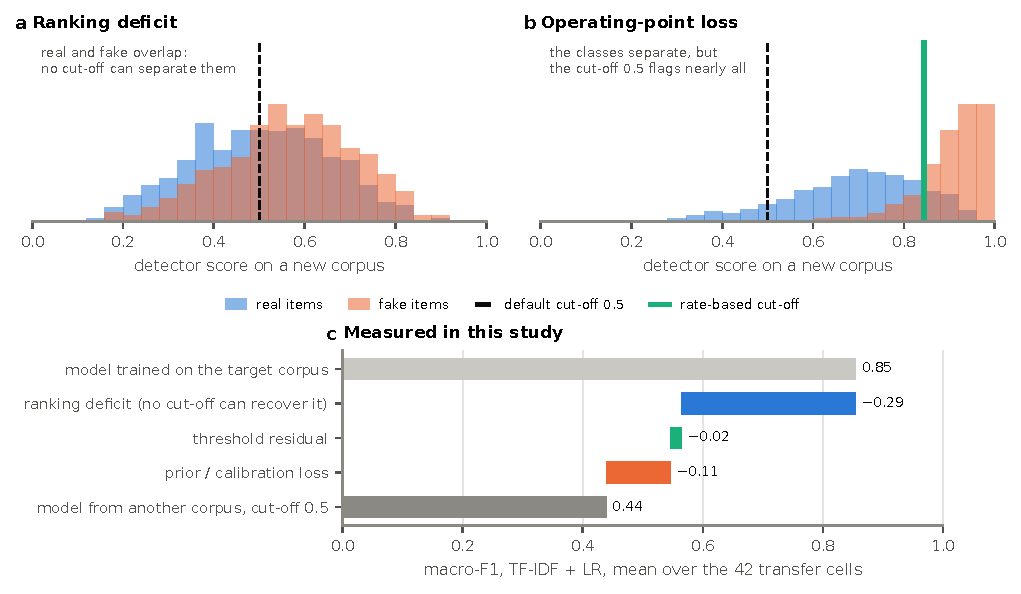
\includegraphics[width=\linewidth]{fig_concept}
\caption{Two ways a detector can fail on a new corpus. (a)~A ranking deficit: real and fake items receive overlapping scores, so no cut-off separates them. (b)~An operating-point loss: the scores separate the classes, but the cut-off learned on the training corpus (0.5) flags almost every item; a cut-off chosen by rate recovers most of the loss. Panels a and b use illustrative simulated scores. (c)~The measured decomposition of Eq.~\eqref{eq:decomp} for TF-IDF with logistic regression, averaged over the 42 transfer cells and five seeds.}\label{fig:concept}
\end{figure}

Two details of Eq.~\eqref{eq:decomp} could bias the split, and we check both. First, the ranking term compares the transfer oracle with the in-domain model at its \emph{default} threshold, so it also contains the in-domain threshold slack $F_{BB}(\tau^\star_{BB})-F_{BB}(\tau_0)$. Second, $\tau^\star$ is chosen on the same items it is scored on, which flatters $F_{AB}(\tau^\star)$ on small test sets and so inflates the operating-point share. We report the slack, and we recompute the decomposition with a \emph{cross-fitted} oracle, whose threshold is tuned on a random half of the target test set and scored on the other half (five repeats, both halves). We also repeat the decomposition with balanced accuracy, which, unlike macro-F1, does not depend on the class prior.

\subsection{Label-free operating points}\label{sec:oprepair}
We compare four ways of choosing a threshold without target labels.
(a)~\emph{EM prior adaptation} \citep{saerens2002adjusting} re-estimates the target prior from the source-calibrated posteriors by expectation--maximisation, adjusts the posteriors and thresholds them at 0.5. With Platt-calibrated scores this is the bias-corrected recipe recommended by \citet{alexandari2020labelshift}, and it is optimal under pure label shift.
(b)~\emph{Rate transfer} sets the threshold so that the share of target items flagged equals the source base rate $\pi_A$. It transfers the model's ranking-based decision rule rather than its score scale. We also report the variant that flags the share $q_A$ the source model flags on its own held-out test split.
(c)~\emph{Adjusted classify-and-count} \citep{forman2008quantifying} estimates the target prior as $\hat\pi_B=(\hat r_B-\mathrm{FPR}_A)/(\mathrm{TPR}_A-\mathrm{FPR}_A)$, where $\hat r_B$ is the share of target items above 0.5 and the error rates come from the source test split, and then flags the top $\hat\pi_B$ of target items.
(d)~A \emph{two-component Gaussian mixture} on the target logits places the threshold where the components' posteriors cross.
As references, we report the share $0.5$, which needs no information at all, and the true target prior $\pi_B$, which needs one number about the target but no item labels.

Rate transfer is a quantile threshold, and quantile thresholds are an old idea in quantification \citep{forman2008quantifying}. We do not claim the rule as new. What matters here is \emph{when} it should beat EM, and that can be stated exactly. Let $F^A_y$ and $F^B_y$ be the distributions of the source model's scores for class $y$ on source and target.

\begin{proposition}\label{prop:rate}
Suppose (i) there is a strictly increasing map $g$ with $F^B_y(g(u))=F^A_y(u)$ for both classes and all $u$, and (ii) $\pi_B=\pi_A$. Then flagging the top $q_A$ share of target items reproduces on $B$ the true- and false-positive rates that the threshold $\tau_0$ has on $A$, whereas the fixed threshold $\tau_0$ does so only if $g(\tau_0)=\tau_0$. If instead $g$ is the identity and $\pi_B\neq\pi_A$ (pure label shift), EM prior adaptation with calibrated scores is consistent and rate transfer is not.
\end{proposition}

The proof is in \ref{app:proof}. The two rules thus suit two different kinds of shift. EM assumes the score distributions within each class stay fixed while the class balance changes. Rate transfer assumes the reverse: the class balance stays roughly fixed while the scores are distorted by an order-preserving map. When the distortion is not order-preserving, part of the loss becomes a ranking deficit that no threshold can recover, which is the first term of Eq.~\eqref{eq:decomp}. Section~\ref{sec:op} checks which assumption our corpora come closer to, and a controlled experiment maps what happens when (ii) fails: each target test set is resampled (1{,}000 items, three draws) to a base rate of $\pi_A+\delta$ for $\delta\in\{-0.3,\dots,0.3\}$, clipped to $[0.05,0.95]$, and every operating point is recomputed.

\subsection{Mechanism probes}\label{sec:probes}
To identify what signal carries in-domain performance, we use eight probes, each run with \textsc{tfidf-lr} unless stated:
\emph{surface statistics only} (\textsc{style-gb} above);
\emph{group-only}, out-of-fold smoothed target encoding of group identity (publisher domain for PolitiFact, GossipCop and BanglaBait; speaker for LIAR; event for PHEME), i.e.\ how well the label is predicted by \emph{who} published an item;
\emph{learning curves} from 32 training items to the full split;
\emph{top-$K$ deletion}, removing the $K\in\{10,\dots,3000\}$ highest-$|w|$ features and retraining \citep[cf.][]{verma2026audit};
\emph{masking} of source tags and datelines, of time expressions and numbers, of named entities (spaCy \texttt{en\_core\_web\_sm}), or of all three;
\emph{topic-balanced training}, where classes are subsampled to equal size inside each of 50 $k$-means topic clusters, removing topic--label correlation from the training set;
\emph{corpus separability}, the proxy $\mathcal{A}$-distance $2(1-2\epsilon)$ between two corpora, with $\epsilon$ the cross-validated error of a classifier that tells them apart from text alone \citep{bendavid2010theory};
and \emph{feature attribution}, the largest-weight n-grams per class and their linear-SHAP magnitudes $|w_j|\,\mathbb{E}|x_j-\bar x_j|$.
For the more expensive probes (top-$K$, masking, vocabulary ablation) training is capped at 4{,}000 and test at 1{,}500 items; masking and vocabulary ablation use three seeds.

\subsection{Representation repairs}\label{sec:repair}
The ranking deficit can only be reduced by a better representation. We test repairs in a leave-one-corpus-out (LOCO) setting: for each held-out veracity corpus, the model is trained on the union of the other six (each capped at 1{,}500 training and 300 validation items) and evaluated on the held-out test split, with near-duplicates of any training corpus removed. Methods are: \emph{pooled} training; pooled training with sample weights that equalise every (corpus, class) cell (\emph{balanced}); balanced training on texts with source tags, datelines, URLs, handles and time expressions \emph{masked}; balanced training after deleting the 2{,}000 features most predictive of \emph{corpus identity} (from a one-vs-rest corpus classifier); and three dense variants on a 300-d SVD of the TF-IDF space: the SVD baseline, \emph{INLP} \citep{ravfogel2020inlp}, which projects out 15 iterations of linear corpus-identity directions, and \emph{CORAL} \citep{sun2016coral}, which aligns source feature covariance to the (unlabelled) target. None uses target labels; CORAL alone uses unlabelled target text.

We also re-implement three published generalisation methods for fake-news detection on one shared backbone, the frozen RoBERTa vectors of the 1{,}500-item subsets, in the same leave-one-corpus-out design (three seeds): EANN-style adversarial training, in which a corpus discriminator behind a gradient-reversal layer removes corpus information from a two-layer encoder \citep{wang2018eann,ganin2016dann}; an MDFEND-style mixture of five expert networks combined by a learned gate \citep{nan2021mdfend}, fed the text vector because the domain of a new corpus is unknown; and ENDEF-style entity debiasing, in which an entity-only model over the named entities found by spaCy is trained jointly with the main model and dropped at test time \citep{zhu2022endef}. Pooled logistic regression and a pooled two-layer network on the same vectors are the references. All networks are trained with AdamW and early stopping on pooled validation AUC.

\section{Results}\label{sec:results}

\subsection{The size of the gap}\label{sec:gap}
Table~\ref{tab:headline} and Figure~\ref{fig:heatmap} summarise the seven-corpus veracity matrix. With \textsc{tfidf-lr}, mean in-domain ROC-AUC is \InAUC{}, mean off-diagonal AUC is \OffAUC{}, and on the eight same-task cells it is \PairAUC{}. The sanity controls behave as they should. With permuted labels, transfer AUC is \PermAUC{} ($\pm$\PermAUCsd{} across cells and seeds) and in-domain AUC \PermInAUC{}. With every source cut to 250 training items the gap remains (in-domain \MatchedInAUC{}, off-diagonal \MatchedOffAUC{}), so it does not come from the very different corpus sizes.

The gap is real, but it is not a collapse to chance. On the cleanest pair, ISOT$\to$WELFake, AUC is \pairISOTWELFakeAUC{} \pairISOTWELFakeCI{}, and in the reverse direction \pairWELFakeISOTAUC{} \pairWELFakeISOTCI{} (Table~\ref{tab:pairs}). Two pairs carry almost no transferable ranking: PolitiFact$\to$LIAR (\pairPFLIARAUC{} \pairPFLIARCI{}) and LIAR$\to$PolitiFact (\pairLIARPFAUC{} \pairLIARPFCI{}). Both are labelled by the same fact-checker, but one rates claims and the other news stories. In \NcellsBelowHalf{} of the 42 off-diagonal cells (\CellsBelowHalf) the mean AUC is below 0.5, meaning that the cue a source teaches points the wrong way on that target.

\begin{table}[t]
\centering
\caption{In-domain versus transfer performance on the seven veracity corpora (mean $\pm$ s.d.\ over seeds of the per-seed mean over cells). ``Pairs'' averages the eight directed same-task cells. Off-diagonal macro-F1 is given at the default threshold and at the oracle threshold. \textsc{roberta-lr} is evaluated on the 1{,}500-item subsets and \textsc{roberta-ft} on 800 training and 300 test items per corpus with three seeds (Section~\ref{sec:models}); compare each with its paired \textsc{tfidf-lr} in Section~\ref{sec:models-res}, not with the rows above.}\label{tab:headline}
\small
\setlength{\tabcolsep}{4pt}
\begin{tabular}{@{}llcccccc@{}}
\toprule
 & & \multicolumn{3}{c}{ROC-AUC} & \multicolumn{3}{c}{macro-F1} \\
\cmidrule(lr){3-5}\cmidrule(lr){6-8}
Model & Regime & In-domain & Off-diag. & Pairs & In-domain & Off-diag. & Off-diag.\ oracle \\
\midrule
\textsc{tfidf-lr} & full & 0.914\,{\scriptsize$\pm$0.006} & 0.567\,{\scriptsize$\pm$0.006} & 0.624\,{\scriptsize$\pm$0.004} & 0.854\,{\scriptsize$\pm$0.005} & 0.439\,{\scriptsize$\pm$0.011} & 0.565\,{\scriptsize$\pm$0.004} \\
\textsc{tfidf-lr} & matched & 0.861\,{\scriptsize$\pm$0.010} & 0.556\,{\scriptsize$\pm$0.004} & 0.590\,{\scriptsize$\pm$0.009} & 0.786\,{\scriptsize$\pm$0.012} & 0.446\,{\scriptsize$\pm$0.014} & 0.558\,{\scriptsize$\pm$0.002} \\
\textsc{tfidf-lr} & permuted & 0.519\,{\scriptsize$\pm$0.026} & 0.499\,{\scriptsize$\pm$0.012} & 0.514\,{\scriptsize$\pm$0.019} & 0.397\,{\scriptsize$\pm$0.014} & 0.377\,{\scriptsize$\pm$0.015} & 0.518\,{\scriptsize$\pm$0.007} \\
\addlinespace
\textsc{tfidf-svm} & full & 0.914\,{\scriptsize$\pm$0.005} & 0.564\,{\scriptsize$\pm$0.005} & 0.625\,{\scriptsize$\pm$0.005} & 0.855\,{\scriptsize$\pm$0.005} & 0.437\,{\scriptsize$\pm$0.009} & 0.564\,{\scriptsize$\pm$0.004} \\
\textsc{tfidf-svm} & matched & 0.862\,{\scriptsize$\pm$0.010} & 0.554\,{\scriptsize$\pm$0.005} & 0.592\,{\scriptsize$\pm$0.010} & 0.787\,{\scriptsize$\pm$0.011} & 0.447\,{\scriptsize$\pm$0.017} & 0.556\,{\scriptsize$\pm$0.003} \\
\textsc{tfidf-svm} & permuted & 0.519\,{\scriptsize$\pm$0.024} & 0.498\,{\scriptsize$\pm$0.015} & 0.511\,{\scriptsize$\pm$0.020} & 0.398\,{\scriptsize$\pm$0.009} & 0.377\,{\scriptsize$\pm$0.012} & 0.516\,{\scriptsize$\pm$0.008} \\
\addlinespace
\textsc{nb-svm} & full & 0.912\,{\scriptsize$\pm$0.004} & 0.547\,{\scriptsize$\pm$0.006} & 0.590\,{\scriptsize$\pm$0.011} & 0.853\,{\scriptsize$\pm$0.008} & 0.410\,{\scriptsize$\pm$0.008} & 0.555\,{\scriptsize$\pm$0.003} \\
\textsc{nb-svm} & matched & 0.862\,{\scriptsize$\pm$0.011} & 0.540\,{\scriptsize$\pm$0.006} & 0.559\,{\scriptsize$\pm$0.004} & 0.786\,{\scriptsize$\pm$0.012} & 0.398\,{\scriptsize$\pm$0.013} & 0.549\,{\scriptsize$\pm$0.004} \\
\textsc{nb-svm} & permuted & 0.510\,{\scriptsize$\pm$0.023} & 0.494\,{\scriptsize$\pm$0.009} & 0.502\,{\scriptsize$\pm$0.009} & 0.400\,{\scriptsize$\pm$0.003} & 0.383\,{\scriptsize$\pm$0.012} & 0.520\,{\scriptsize$\pm$0.006} \\
\addlinespace
\textsc{glove-lr} & full & 0.864\,{\scriptsize$\pm$0.005} & 0.564\,{\scriptsize$\pm$0.005} & 0.610\,{\scriptsize$\pm$0.005} & 0.782\,{\scriptsize$\pm$0.007} & 0.465\,{\scriptsize$\pm$0.004} & 0.564\,{\scriptsize$\pm$0.004} \\
\textsc{glove-lr} & matched & 0.830\,{\scriptsize$\pm$0.006} & 0.563\,{\scriptsize$\pm$0.010} & 0.592\,{\scriptsize$\pm$0.017} & 0.740\,{\scriptsize$\pm$0.011} & 0.466\,{\scriptsize$\pm$0.010} & 0.564\,{\scriptsize$\pm$0.007} \\
\textsc{glove-lr} & permuted & 0.520\,{\scriptsize$\pm$0.022} & 0.504\,{\scriptsize$\pm$0.026} & 0.494\,{\scriptsize$\pm$0.021} & 0.404\,{\scriptsize$\pm$0.020} & 0.391\,{\scriptsize$\pm$0.012} & 0.525\,{\scriptsize$\pm$0.019} \\
\addlinespace
\textsc{style-gb} & full & 0.745\,{\scriptsize$\pm$0.009} & 0.535\,{\scriptsize$\pm$0.004} & 0.595\,{\scriptsize$\pm$0.008} & 0.679\,{\scriptsize$\pm$0.005} & 0.427\,{\scriptsize$\pm$0.007} & 0.548\,{\scriptsize$\pm$0.003} \\
\textsc{style-gb} & matched & 0.702\,{\scriptsize$\pm$0.008} & 0.526\,{\scriptsize$\pm$0.009} & 0.561\,{\scriptsize$\pm$0.032} & 0.632\,{\scriptsize$\pm$0.008} & 0.413\,{\scriptsize$\pm$0.017} & 0.542\,{\scriptsize$\pm$0.007} \\
\textsc{style-gb} & permuted & 0.503\,{\scriptsize$\pm$0.018} & 0.502\,{\scriptsize$\pm$0.016} & 0.493\,{\scriptsize$\pm$0.028} & 0.410\,{\scriptsize$\pm$0.008} & 0.390\,{\scriptsize$\pm$0.007} & 0.523\,{\scriptsize$\pm$0.011} \\
\addlinespace
\textsc{roberta-lr} & full & 0.861\,{\scriptsize$\pm$0.012} & 0.544\,{\scriptsize$\pm$0.008} & 0.630\,{\scriptsize$\pm$0.011} & 0.777\,{\scriptsize$\pm$0.013} & 0.452\,{\scriptsize$\pm$0.013} & 0.549\,{\scriptsize$\pm$0.010} \\
\addlinespace
\textsc{roberta-ft} & full & 0.867\,{\scriptsize$\pm$0.010} & 0.559\,{\scriptsize$\pm$0.013} & 0.614\,{\scriptsize$\pm$0.020} & 0.795\,{\scriptsize$\pm$0.005} & 0.418\,{\scriptsize$\pm$0.009} & 0.571\,{\scriptsize$\pm$0.008} \\
\bottomrule
\end{tabular}
\end{table}


\begin{figure}[t]
\centering
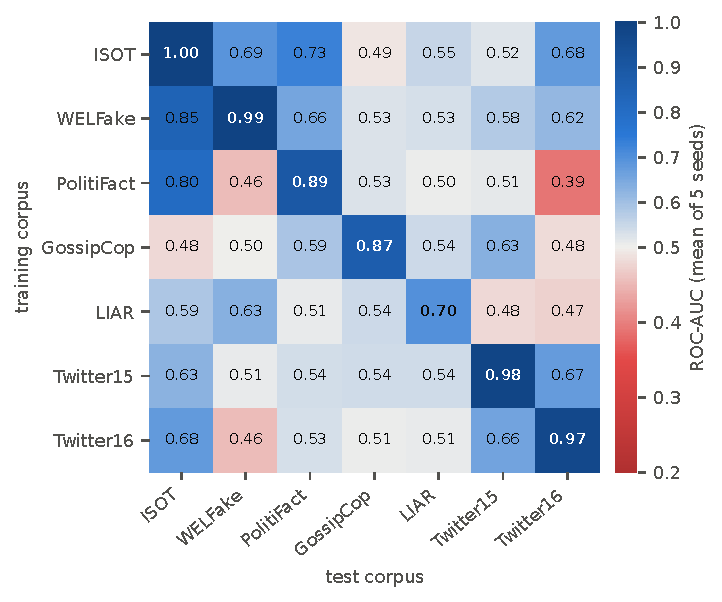
\includegraphics[width=0.62\linewidth]{fig_heatmap_auc}
\caption{Transfer ROC-AUC of \textsc{tfidf-lr} (mean of five seeds). Rows are training corpora, columns test corpora; the diagonal is in-domain. Blue is above chance, red below; the midpoint is 0.5.}\label{fig:heatmap}
\end{figure}

\begin{table}[t]
\centering
\caption{Same-task pairs (\textsc{tfidf-lr}, five seeds). AUC with pooled seed-bootstrap 95\% CI; ``In'' is the source's in-domain AUC; prior is the target fake rate and PPR the predicted-positive rate at $t=0.5$; macro-F1 at the default, prior-matched and oracle thresholds; ECE of the source-calibrated scores on the target.}\label{tab:pairs}
\small
\begin{tabular}{@{}lcccccccc@{}}
\toprule
Pair & In & AUC [95\% CI] & Prior & PPR & F1$_{0.5}$ & F1$_{\pi}$ & F1$^\star$ & ECE \\
\midrule
ISOT$\to$WELFake & 0.999 & 0.690 [0.66, 0.71] & 0.43 & 0.78 & 0.539 & 0.635 & 0.638 & 0.38 \\
WELFake$\to$ISOT & 0.989 & 0.847 [0.82, 0.87] & 0.46 & 0.36 & 0.753 & 0.763 & 0.765 & 0.11 \\
PolitiFact$\to$GossipCop & 0.893 & 0.526 [0.48, 0.56] & 0.23 & 0.54 & 0.464 & 0.514 & 0.517 & 0.32 \\
GossipCop$\to$PolitiFact & 0.869 & 0.589 [0.50, 0.68] & 0.43 & 0.07 & 0.425 & 0.576 & 0.595 & 0.28 \\
Twitter15$\to$Twitter16 & 0.981 & 0.672 [0.52, 0.82] & 0.46 & 0.62 & 0.572 & 0.597 & 0.646 & 0.25 \\
Twitter16$\to$Twitter15 & 0.967 & 0.657 [0.55, 0.75] & 0.51 & 0.63 & 0.580 & 0.591 & 0.631 & 0.28 \\
LIAR$\to$PolitiFact & 0.698 & 0.508 [0.42, 0.60] & 0.44 & 0.54 & 0.495 & 0.517 & 0.536 & 0.12 \\
PolitiFact$\to$LIAR & 0.893 & 0.505 [0.47, 0.54] & 0.44 & 0.40 & 0.497 & 0.502 & 0.509 & 0.22 \\
\bottomrule
\end{tabular}
\end{table}


Threshold-dependent metrics look much worse than AUC. Off-diagonal macro-F1 at the default threshold averages \OffFone{}, not far above the one-class level of 0.33, against \InFone{} in-domain. The predicted-positive rates in Table~\ref{tab:pairs} show why. An ISOT model flags \pairISOTWELFakePPR{} of WELFake as fake although the fake rate is \pairISOTWELFakePrior{}, and a GossipCop model flags only \pairGCPFPPR{} of PolitiFact although its fake rate is \pairGCPFPrior{}. Scores that were well calibrated in-domain are badly calibrated on the target.

\subsection{Where the gap goes}\label{sec:where}
Applying Eq.~\eqref{eq:decomp} cell by cell (Table~\ref{tab:decomp}, Figure~\ref{fig:decomp}) splits the loss into a part that no threshold can recover and a part that the right threshold would. For \textsc{tfidf-lr} on the same-task pairs, the mean transfer gap is \GapPair{} macro-F1 points, of which \RankPair{} (\RankSharePair) is a ranking deficit and the rest an operating-point loss. On the other cells the gap is \GapOther{}, and \RankShareOther{} of it is ranking. Over all cells, \RankShareAll{} of the loss is ranking (corpus-bootstrap 95\% interval \RankShareCI) and \OpShareAll{} is operating point. Most of the gap is ranking, then, and part of it is threshold. Both parts matter. The operating-point share is large enough to change which of two detectors looks better, and it is the cheaper one to fix.

\begin{table}[t]
\centering
\caption{Transfer gap decomposition (Eq.~\ref{eq:decomp}), macro-F1 points, mean over cells and seeds. The gap is relative to the target's own in-domain score.}\label{tab:decomp}
\small
\begin{tabular}{@{}llrrrrr@{}}
\toprule
Model & Cells & Gap & Ranking & Threshold & Prior/cal. & Ranking share \\
\midrule
\textsc{tfidf-lr} & pairs & 0.308 & 0.244 & 0.018 & 0.046 & 79\% \\
\textsc{tfidf-lr} & other cells & 0.441 & 0.300 & 0.018 & 0.122 & 68\% \\
\textsc{tfidf-svm} & pairs & 0.308 & 0.243 & 0.016 & 0.049 & 79\% \\
\textsc{tfidf-svm} & other cells & 0.444 & 0.303 & 0.018 & 0.123 & 68\% \\
\textsc{nb-svm} & pairs & 0.319 & 0.261 & 0.023 & 0.036 & 82\% \\
\textsc{nb-svm} & other cells & 0.472 & 0.306 & 0.021 & 0.145 & 65\% \\
\textsc{glove-lr} & pairs & 0.281 & 0.193 & 0.016 & 0.071 & 69\% \\
\textsc{glove-lr} & other cells & 0.327 & 0.224 & 0.017 & 0.085 & 69\% \\
\textsc{style-gb} & pairs & 0.141 & 0.091 & 0.013 & 0.036 & 65\% \\
\textsc{style-gb} & other cells & 0.278 & 0.141 & 0.020 & 0.117 & 51\% \\
\textsc{roberta-lr} & pairs & 0.243 & 0.162 & 0.022 & 0.059 & 66\% \\
\textsc{roberta-lr} & other cells & 0.344 & 0.244 & 0.024 & 0.076 & 71\% \\
\textsc{roberta-ft} & pairs & 0.340 & 0.186 & 0.031 & 0.123 & 55\% \\
\textsc{roberta-ft} & other cells & 0.387 & 0.233 & 0.027 & 0.127 & 60\% \\
\bottomrule
\end{tabular}
\end{table}


\begin{figure}[t]
\centering
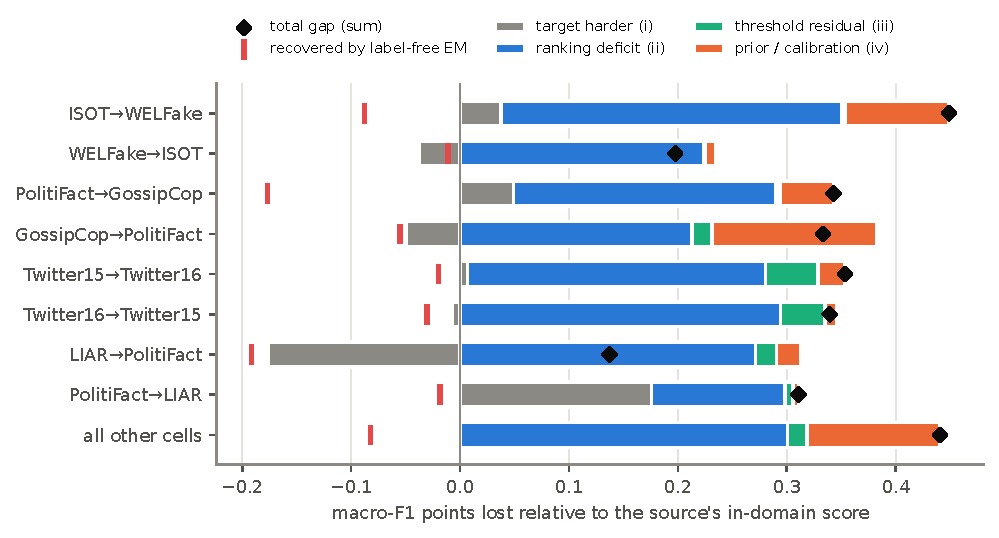
\includegraphics[width=\linewidth]{fig_gap_decomposition}
\caption{Transfer gap decomposition for \textsc{tfidf-lr} (macro-F1 points relative to the source's in-domain score, mean of five seeds). Grey: target harder or easier than source; blue: ranking deficit; green and orange: operating-point losses. Diamonds mark the total; red ticks show what EM prior adaptation recovers (negative values make things worse).}\label{fig:decomp}
\end{figure}

\subsection{How robust is the split?}\label{sec:robust}
The split survives every check we ran. Dropping any one corpus from the matrix leaves the ranking share between \RankShareDropMin{} and \RankShareDropMax. The in-domain threshold slack that the ranking term absorbs is small, \SlackFone{} macro-F1 on average (at most \SlackFoneMax). The in-sample oracle is optimistic, as expected: a threshold tuned on one half of the target and scored on the other reaches \OracleCF{}, which is \OracleCFbias{} below the in-sample oracle on average and \OracleCFbiasSmall{} below it on the targets with fewer than 250 test items. With the cross-fitted oracle the ranking share rises to \RankShareCF{}, so if anything Eq.~\eqref{eq:decomp} overstates the operating-point part. With balanced accuracy in place of macro-F1, the ranking share is \BARankShare{}. Across detectors the ranking share varies more (Table~\ref{tab:decomp}): it is lowest for the style model on the non-paired cells and for the fine-tuned transformer (\FTRankShare{} overall; Section~\ref{sec:models-res}), but ranking is the larger part for every detector.

\subsection{Repairing the operating point without labels}\label{sec:op}
Table~\ref{tab:oppoints} and Figure~\ref{fig:op} compare operating points. EM prior adaptation, the textbook remedy, \emph{lowers} off-diagonal macro-F1 from \OPDef{} to \OPEM{}. It recovers \RecEM{} of the operating-point loss (interval \RecEMCI), and it does so for every detector (\RecEMMin{} to \RecEMMax). Rate transfer, which flags the same share of target items as the source base rate, raises macro-F1 to \OPRank{} and recovers \RecRank{} (\RecRankCI), close to the \RecPrior{} reached when the true target base rate is known (\OPPrior{}). It recovers between \RecRankMin{} and \RecRankMax{} across the seven detectors, and it is at least as good as the cross-fitted oracle, that is, as a threshold tuned on half of the labelled target set (recovery \RecRankCF{} against that oracle). Flagging the share $q_A$ that the source model flags in-domain recovers \RecSrcPPR, and the mixture model \RecGMM. Rate transfer is worse than the default threshold in \RankWorseShare{} of the cell-seed combinations.

Two observations keep these numbers in proportion. First, flagging exactly half of the items recovers \RecHalf{}, almost as much as rate transfer. The source base rates of our corpora lie between 0.23 and 0.51, so in this benchmark most of the gain comes from switching from a score threshold to \emph{any} sensible rate threshold, and only a small part from knowing the source rate. Second, the source base rate is a good guess of the target base rate here (mean absolute error \SrcPriorErr), which is condition (ii) of Proposition~\ref{prop:rate}.

Why does EM fail? The answer is in the calibration. EM is optimal when only $p(y)$ changes and calibrated posteriors stay meaningful. Here calibration does not survive the move: expected calibration error is \ECEin{} in-domain but \ECEout{} on the target. EM's prior estimates therefore drift towards 0 or 1 (mean absolute error \EMpriorErr), far worse than simply assuming the source prior (\SrcPriorErr). Adjusted classify-and-count fails for the same reason, because the source error rates it inverts do not hold on the target either (prior error \ErrACC, recovery \RecACC). The shift is in $p(x\mid y)$, that is, in style, topic and source, much more than in $p(y)$. That is the regime in which Proposition~\ref{prop:rate} favours transferring the rate over transferring the scores.

\begin{table}[t]
\centering
\caption{Off-diagonal macro-F1 under different operating points (mean over the 42 cells and five seeds). Label-free: default $t=0.5$, EM prior adaptation, rate transfer (predicted-positive rate set to the source base rate), predicted-positive rate 0.5, and a 2-component GMM on target logits. With one number known: rate set to the true target prior. Upper bound: oracle threshold. For \textsc{tfidf-lr}, Holm-corrected Wilcoxon $p$ versus default: EM 1.6e-32, rate transfer 6.6e-31, rate 0.5 1.4e-29, GMM 1.7e-18.}\label{tab:oppoints}
\small
\begin{tabular}{@{}lccccccc@{}}
\toprule
 & \multicolumn{5}{c}{label-free} & prior known & bound \\
\cmidrule(lr){2-6}\cmidrule(lr){7-7}\cmidrule(lr){8-8}
Model & $t=0.5$ & EM & rate transfer & rate 0.5 & GMM & rate $=\pi_B$ & oracle \\
\midrule
\textsc{tfidf-lr} & 0.439 & 0.358 & 0.541 & 0.539 & 0.510 & 0.547 & 0.565 \\
\textsc{tfidf-svm} & 0.437 & 0.363 & 0.539 & 0.537 & 0.503 & 0.546 & 0.564 \\
\textsc{nb-svm} & 0.410 & 0.349 & 0.525 & 0.526 & 0.444 & 0.534 & 0.555 \\
\textsc{glove-lr} & 0.465 & 0.381 & 0.540 & 0.542 & 0.494 & 0.547 & 0.564 \\
\textsc{style-gb} & 0.427 & 0.347 & 0.521 & 0.521 & 0.477 & 0.529 & 0.548 \\
\textsc{roberta-lr} & 0.452 & 0.368 & 0.516 & 0.516 & 0.477 & 0.525 & 0.549 \\
\textsc{roberta-ft} & 0.418 & 0.340 & 0.535 & 0.534 & 0.479 & 0.544 & 0.571 \\
\bottomrule
\end{tabular}
\end{table}


\begin{figure}[t]
\centering
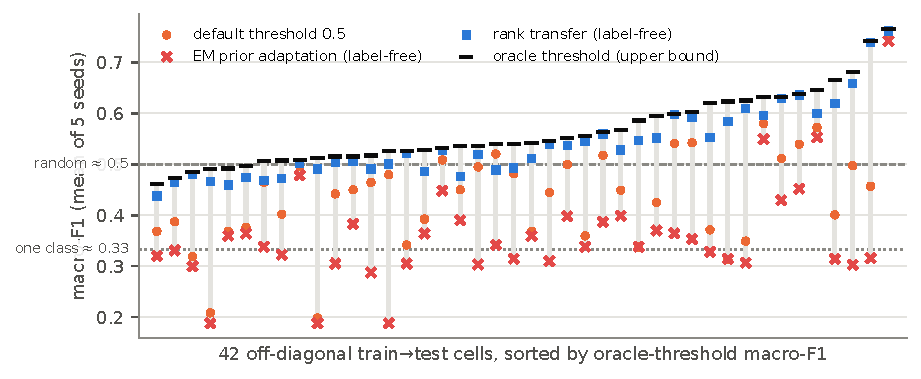
\includegraphics[width=\linewidth]{fig_operating_points}
\caption{Off-diagonal macro-F1 of \textsc{tfidf-lr} for each of the 42 cells (mean of five seeds), sorted by the oracle bound. Rate transfer closes most of the distance from the default threshold to the oracle without any target label; EM prior adaptation often falls below the default.}\label{fig:op}
\end{figure}

\paragraph{When the base rate moves}
Condition (ii) will not always hold, so we resampled every target to base rates between 0.3 below and 0.3 above the source rate (Figure~\ref{fig:priorshift}). Rate transfer degrades as the shift grows: it recovers \PSrecZero{} of the operating-point loss with no shift, \PSrecMinus{} at $-0.3$ and \PSrecPlus{} at $+0.3$, where its macro-F1 (\PSrankPlus) falls well below that of a threshold set at the true rate (\PStruePlus). It still beats the default threshold at every shift we tried, by \PSgainMin{} to \PSgainMax{} macro-F1. The two label-free prior estimators do not help: EM and adjusted classify-and-count stay below the default threshold at every shift, because both rely on score distributions that do not transfer. In practice, then, rate transfer is a safe default, but when the base rate of the new feed is expected to differ from the training data, an estimate of that rate from a small labelled sample is worth more than any label-free correction we tested.

\begin{figure}[t]
\centering
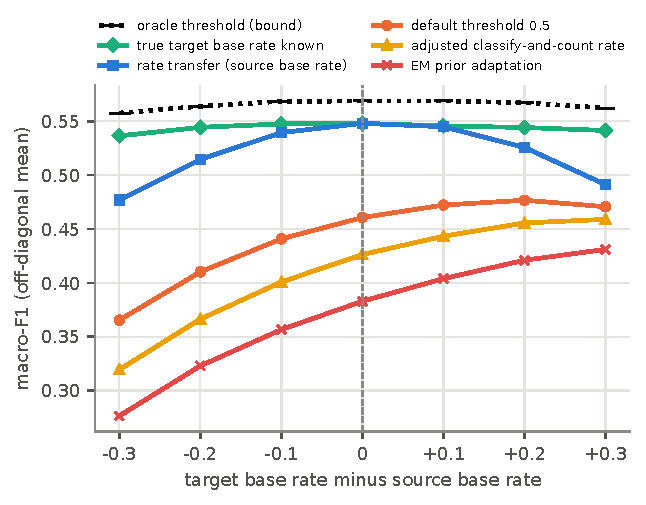
\includegraphics[width=0.66\linewidth]{fig_prior_shift}
\caption{Off-diagonal macro-F1 of \textsc{tfidf-lr} when every target test set is resampled to the source base rate plus a shift (42 cells, five seeds, three draws of 1{,}000 items). Rate transfer is best when the base rate is unchanged and degrades as it moves; the label-free prior estimators (EM, adjusted classify-and-count) stay below the default threshold throughout.}\label{fig:priorshift}
\end{figure}

\subsection{The gap across models}\label{sec:models-res}
The picture does not depend on the detector (Table~\ref{tab:headline}; full matrices for every model are in the Supplementary Material). The four content models reach in-domain AUC between \InAUCmin{} and \InAUCmax{} and off-diagonal AUC between \OffAUCmin{} and \OffAUCmax{}, and all of them show the same split between ranking and operating-point loss (Table~\ref{tab:decomp}). Averaged word embeddings (\textsc{glove-lr}) are weaker in-domain (\GloveInAUC) and transfer no better (\GloveOffAUC).

The style model is the most revealing. With only 22 surface statistics it reaches an average in-domain AUC of \StyleInAUC{} (\StyleISOT{} on ISOT, \StyleWEL{} on WELFake), and its transfer AUC (\StyleOffAUC) is only a few points below that of the lexical models. A large part of what these benchmarks reward is form: length, casing, punctuation and attribution habits (Section~\ref{sec:shortcuts}).

Pretrained encoders do not change the conclusion. On identical 1{,}500-item subsets, frozen RoBERTa features give in-domain AUC \RobInAUC{} and off-diagonal AUC \RobOffAUC{}, against \SubLRInAUC{} and \SubLROffAUC{} for \textsc{tfidf-lr} refitted on the same splits. The paired off-diagonal difference is \RobMinusLRoff{} AUC (Wilcoxon $p=\RobMinusLRp$), and RoBERTa is better in \RobBetterCells{} of the 42 cells. Fine-tuning the upper four layers does not change this either. On the same 800 training and 300 test items per corpus (\FTseeds{} seeds), \textsc{roberta-ft} reaches in-domain AUC \FTInAUC{} and off-diagonal AUC \FTOffAUC{}, against \FTsubInAUC{} and \FTsubOffAUC{} for the paired \textsc{tfidf-lr}; the off-diagonal difference is \FTminusLRoff{} (Wilcoxon $p=\FTminusLRp$, better in \FTbetterCells{} of 42 cells). Its gap is again mostly ranking (\FTRankShare), EM again makes the operating point worse (\FTRecEM{} recovered), and rate transfer again recovers most of it (\FTRecRank). With only four layers trained on 800 items, the fine-tuned model is slightly weaker than \textsc{tfidf-lr} in-domain (\FTminusLRin{} AUC), so this is not the strongest transformer one could build; but its transfer matches that of the lexical model, and the shape of its gap is the same. This agrees with \citet{verma2026audit} and \citet{delloglio2026comparison}, who found that fully fine-tuned transformers gain in-domain but not, or not reliably, across corpora. Pairwise McNemar tests on the same target items (Holm-corrected over all comparisons) find significant differences from \textsc{tfidf-lr} in the following share of (cell, seed) comparisons: \McFracSig.

\subsection{What the detectors learn}\label{sec:shortcuts}
\paragraph{Cheap signals go a long way}
Table~\ref{tab:shortcuts} lists four shortcut indicators per corpus. The surface-statistics model recovers on average \StyleShare{} of the above-chance in-domain AUC of the full lexical model, and on the article corpora almost all of it (ISOT \StyleISOT, WELFake \StyleWEL). Sixty-four training examples are enough for an in-domain AUC of \LCsixfourISOT{} on ISOT and \LCsixfourWEL{} on WELFake; the claim and celebrity-headline corpora, whose in-domain scores are lower to begin with, learn much more slowly (LIAR \LCsixfourLIAR, GossipCop \LCsixfourGC). On the headline and claim corpora, publisher or speaker identity alone predicts the label with AUC \GroupPF{} (PolitiFact), \GroupGC{} (GossipCop) and \GroupLIAR{} (LIAR). A label that can be predicted from form, from a few dozen examples or from who published an item is a label whose in-domain score says little about veracity.

\begin{table}[t]
\centering
\caption{Shortcut indicators (ROC-AUC, mean of five seeds). In-domain AUC of \textsc{tfidf-lr} with the full training split, of the surface-statistics \textsc{style-gb}, and of \textsc{tfidf-lr} trained on only 64 or 256 items; AUC of a group-identity baseline (publisher domain for PolitiFact and GossipCop, speaker for LIAR); and the mean off-diagonal AUC with the corpus as source and as target.}\label{tab:shortcuts}
\small
\begin{tabular}{@{}lccccccc@{}}
\toprule
 & \multicolumn{5}{c}{in-domain} & \multicolumn{2}{c}{transfer} \\
\cmidrule(lr){2-6}\cmidrule(lr){7-8}
Corpus & full & style only & $n=64$ & $n=256$ & group only & as source & as target \\
\midrule
ISOT & 0.999 & 0.999 & 0.983 & 0.991 & -- & 0.611 & 0.670 \\
WELFake & 0.989 & 0.951 & 0.894 & 0.941 & -- & 0.626 & 0.540 \\
PolitiFact & 0.893 & 0.787 & 0.742 & 0.850 & 0.840 & 0.533 & 0.592 \\
GossipCop & 0.869 & 0.659 & 0.610 & 0.723 & 0.807 & 0.538 & 0.522 \\
LIAR & 0.698 & 0.590 & 0.567 & 0.607 & 0.664 & 0.537 & 0.530 \\
Twitter15 & 0.981 & 0.603 & 0.793 & 0.962 & -- & 0.572 & 0.563 \\
Twitter16 & 0.967 & 0.625 & 0.890 & -- & -- & 0.556 & 0.552 \\
\bottomrule
\end{tabular}
\end{table}


\paragraph{The strongest cues are collection signatures}
Figure~\ref{fig:weights} shows the highest-weight n-grams. In ISOT, the real class is signalled by Reuters wire conventions (``reuters'', ``said'', ``washington reuters'', weekday attributions such as ``on thursday'') and the fake class by the template of the sites it was collected from (``featured image'', ``image via'', ``read more'', ``video''). In WELFake, the real class is signalled by publisher suffixes inherited from one of its source collections (``breitbart'', ``york times'', ``mr'') and the fake class by the window in which fake items were gathered (``2016'', ``october'', ``november'', ``hillary''). Each corpus thus teaches a different, corpus-specific proxy, which explains why the sign of a cue can flip from one corpus to another (Section~\ref{sec:gap}).

\begin{figure}[t]
\centering
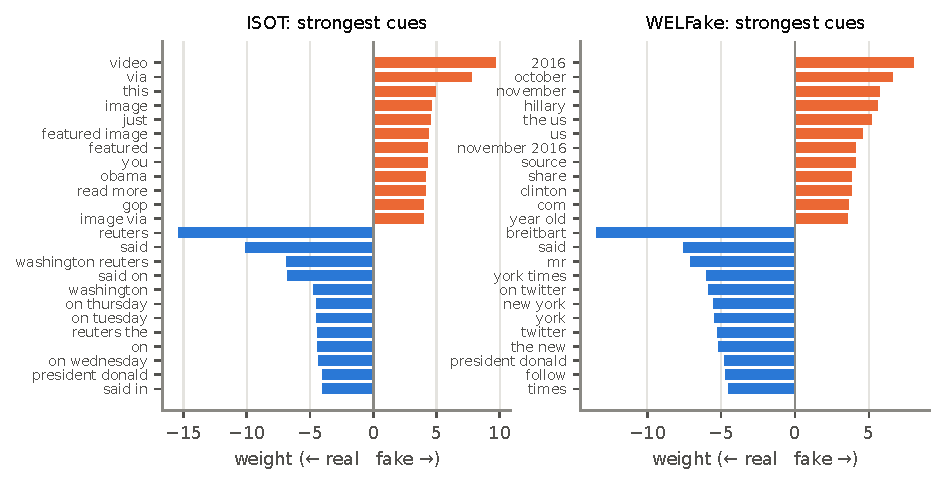
\includegraphics[width=\linewidth]{fig_weights}
\caption{Highest-weight n-grams of \textsc{tfidf-lr} (seed 0) for the real (blue) and fake (orange) classes. Both corpora are separated mainly by outlet conventions and collection-period vocabulary.}\label{fig:weights}
\end{figure}

\paragraph{Removing cues does not remove the signal}
Deleting the top-$K$ features and retraining barely moves in-domain AUC: on ISOT it goes from \TopKISOTIn{} with all features to \TopKISOTInThousand{} after deleting 1{,}000 and \TopKISOTInMax{} after 3{,}000, and on WELFake from \TopKWELIn{} to \TopKWELInThousand{} and \TopKWELInMax{}; transfer to the paired corpus, in contrast, falls from \TopKISOTPair{} to \TopKISOTPairMax{} (ISOT$\to$WELFake) and from \TopKWELPair{} to \TopKWELPairMax{} (WELFake$\to$ISOT). The highest-weight features thus carry most of what transfers, while the signal that keeps in-domain AUC near its ceiling is spread over thousands of corpus-specific features. Masking source tags, datelines, time expressions, numbers and named entities together (Table~\ref{tab:mask}) leaves in-domain AUC at \MaskISOTAllIn{} (ISOT) and \MaskWELAllIn{} (WELFake), and moves ISOT$\to$WELFake from \MaskISOTNonePair{} to \MaskISOTAllPair{} and WELFake$\to$ISOT from \MaskWELNonePair{} to \MaskWELAllPair{}. Balancing classes within each of 50 topic clusters, whose class purity averages \TopicISOTPurity{} in ISOT and \TopicWELPurity{} in WELFake, leaves in-domain AUC unchanged (ISOT \TopicISOTRandIn{}$\to$\TopicISOTBalIn{}, WELFake \TopicWELRandIn{}$\to$\TopicWELBalIn{}) and transfer unchanged (\TopicISOTRandOut{}$\to$\TopicISOTBalOut{}, \TopicWELRandOut{}$\to$\TopicWELBalOut{}); only GossipCop loses in-domain AUC (\TopicGCRandIn{}$\to$\TopicGCBalIn{}). The separating signal is therefore diffuse: it lives in style and register throughout the text, not in a removable list of tokens or topics, as \citet{verma2026audit} also found for ISOT.

\begin{table}[t]
\centering
\caption{Masking ablation (\textsc{tfidf-lr}, ROC-AUC, three seeds, first 3{,}000 characters). Rows: training corpus and what is masked in every corpus; columns: test corpus (the training corpus's own column is in-domain).}\label{tab:mask}
\small
\begin{tabular}{@{}llccccc@{}}
\toprule
Train & Masked & ISOT & WELFake & PolitiFact & GossipCop & LIAR \\
\midrule
ISOT & none & 0.998 & 0.679 & 0.739 & 0.481 & 0.559 \\
ISOT & source tags, datelines, URLs, handles & 0.997 & 0.681 & 0.733 & 0.483 & 0.559 \\
ISOT & dates, weekdays, numbers & 0.998 & 0.692 & 0.723 & 0.479 & 0.563 \\
ISOT & named entities & 0.996 & 0.657 & 0.678 & 0.543 & 0.557 \\
ISOT & all of the above & 0.996 & 0.650 & 0.678 & 0.540 & 0.556 \\
\addlinespace
WELFake & none & 0.808 & 0.980 & 0.636 & 0.529 & 0.532 \\
WELFake & source tags, datelines, URLs, handles & 0.815 & 0.979 & 0.634 & 0.533 & 0.536 \\
WELFake & dates, weekdays, numbers & 0.831 & 0.977 & 0.608 & 0.509 & 0.526 \\
WELFake & named entities & 0.833 & 0.965 & 0.614 & 0.511 & 0.522 \\
WELFake & all of the above & 0.810 & 0.964 & 0.611 & 0.500 & 0.522 \\
\bottomrule
\end{tabular}
\end{table}


\paragraph{Corpus divergence does not predict transfer}
Every pair of corpora can be told apart from text alone (proxy $\mathcal{A}$-distance between \PADmin{} and \PADmax{}, maximum 2; ISOT--WELFake \PADiw), yet across the 42 cells we find no association between source--target divergence and transfer AUC (Spearman $\rho=\PADrho$). With seven corpora the corpus-bootstrap 95\% interval is wide (\PADrhoCI), so a moderate association cannot be excluded, but label-free divergence is clearly not a usable predictor of transfer here. Transfer depends less on how different two corpora look than on whether the cue that separates the classes in one also separates them, with the same sign, in the other.

\subsection{Repairing the ranking}\label{sec:repair-res}
Table~\ref{tab:repair} reports the leave-one-corpus-out repairs (per-target values in Table~\ref{tab:repair-targets}). Training on the six other corpora at once is the one change that helps ranking: held-out AUC rises to \LocoPooled{}, against \LocoMeanSingle{} for the average single source. This is close to the best single source chosen with hindsight (\LocoBestSingle), which cannot be identified without target labels, and far below the targets' own in-domain AUC of \LocoCeiling{}. Nothing we add on top of pooling helps on average. Balancing every (corpus, class) cell (\LocoBal, $\Delta$\LocoBalDelta, $p=\LocoBalP$) and masking collection signatures (\LocoMask, $\Delta$\LocoMaskDelta, $p=\LocoMaskP$) leave AUC unchanged on average; masking helps clearly only on ISOT (Table~\ref{tab:repair-targets}), the corpus whose signatures it was written for.

Methods that make the representation \emph{invariant to corpus identity} make ranking worse: deleting the 2{,}000 most corpus-predictive features gives \LocoDrop{} ($\Delta$\LocoDropDelta, $p=\LocoDropP$), CORAL \LocoCORAL{} ($\Delta$\LocoCORALDelta, $p=\LocoCORALP$) and INLP \LocoINLP{} ($\Delta$\LocoINLPDelta, $p=\LocoINLPP$). INLP does what it is designed to do, reducing linear corpus-identity accuracy from \INLPaccBefore{} to \INLPaccAfter{} (six classes), but it removes veracity information with it. In these benchmarks corpus identity and label are entangled: each corpus collected its fake and real items from different outlets, periods and formats, so the directions that identify a corpus are partly the directions that separate its classes. Invariance to the corpus is therefore not invariance to the shortcut, and the remaining ranking gap is a property of the data rather than of the learner.

\begin{table}[t]
\centering
\caption{Leave-one-corpus-out repairs (\textsc{tfidf-lr} features; mean over the seven held-out veracity corpora and five seeds; s.d.\ across seeds). $\Delta$AUC versus pooled training with Holm-corrected Wilcoxon $p$ over the 35 (target, seed) pairs. For reference, the mean single-source transfer AUC to the same targets is 0.567, the best single source (chosen with target labels) 0.671, and the targets' own in-domain AUC 0.914.}\label{tab:repair}
\small
\begin{tabular}{@{}lccccc@{}}
\toprule
Training & AUC & AP & F1$_{0.5}$ & F1$^\star$ & $\Delta$AUC ($p$) \\
\midrule
pooled (6 corpora) & 0.660\,{\scriptsize$\pm$0.013} & 0.582 & 0.581 & 0.634 & -- \\
+ (corpus, class) balancing & 0.659\,{\scriptsize$\pm$0.013} & 0.583 & 0.582 & 0.632 & -0.001 (1.000) \\
+ balancing + masking & 0.661\,{\scriptsize$\pm$0.012} & 0.584 & 0.576 & 0.633 & +0.001 (1.000) \\
+ balancing + corpus-feature deletion & 0.636\,{\scriptsize$\pm$0.011} & 0.556 & 0.560 & 0.611 & -0.023 (0.006) \\
SVD-300 + balancing & 0.647\,{\scriptsize$\pm$0.009} & 0.566 & 0.583 & 0.624 & -0.013 (0.043) \\
SVD-300 + INLP & 0.605\,{\scriptsize$\pm$0.011} & 0.520 & 0.525 & 0.591 & -0.054 (0.001) \\
SVD-300 + CORAL & 0.621\,{\scriptsize$\pm$0.008} & 0.539 & 0.563 & 0.604 & -0.038 ($<$0.001) \\
\bottomrule
\end{tabular}
\end{table}

\begin{table}[h]
\centering
\caption{Leave-one-corpus-out AUC per held-out corpus (mean of five seeds), against single-source transfer and the in-domain ceiling.}\label{tab:repair-targets}
\small
\begin{tabular}{@{}lccccccc@{}}
\toprule
Held out & mean single & best single & pooled & + masking & INLP & CORAL & in-domain \\
\midrule
ISOT & 0.670 & 0.847 & 0.865 & 0.890 & 0.805 & 0.781 & 0.999 \\
WELFake & 0.540 & 0.690 & 0.648 & 0.657 & 0.643 & 0.643 & 0.989 \\
PolitiFact & 0.592 & 0.730 & 0.677 & 0.655 & 0.600 & 0.650 & 0.893 \\
GossipCop & 0.522 & 0.544 & 0.538 & 0.546 & 0.558 & 0.520 & 0.869 \\
LIAR & 0.530 & 0.552 & 0.528 & 0.528 & 0.502 & 0.514 & 0.698 \\
Twitter15 & 0.563 & 0.657 & 0.647 & 0.645 & 0.592 & 0.626 & 0.981 \\
Twitter16 & 0.552 & 0.678 & 0.715 & 0.703 & 0.536 & 0.616 & 0.967 \\
\bottomrule
\end{tabular}
\end{table}


\subsection{A low-resource language: Bengali clickbait}\label{sec:bangla}
\paragraph{Replication and duplicates}
On the official BanglaBait split, character 3--5-gram logistic regression reaches a clickbait-class F1 of \BBrelFone{} (Figure~\ref{fig:bengali}a), within two points of the 66.28 reported for the same model by \citet{mahtab2023banglabait}, and a linear SVM reaches \BBrelSVMFone{}. Removing the near-duplicates found by MinHash from the official splits lowers the same model to \BBdedFone{} (AUC \BBrelAUC{}$\to$\BBdedAUC{}): even after the original authors' Levenshtein filter, duplicated titles inflate the benchmark. Over five random re-splits of the deduplicated corpus the model reaches AUC \BBseedAUC{} $\pm$ \BBseedAUCsd{}.

\paragraph{Publisher identity}
The \BBnPub{} publishers with at least 100 articles have clickbait rates from \BBrateMin{} to \BBrateMax{}, so publisher identity alone predicts the label with AUC \BBgroupAUC{} (Section~\ref{sec:shortcuts}). Leave-one-publisher-out evaluation nevertheless costs little: across \BBlosoN{} held-out publishers (the smallest ones pooled), mean AUC is \BBlosoAUC{} (range \BBlosoMin--\BBlosoMax), close to the random-split value. Bengali clickbait detection survives a change of source that English veracity detection does not. One reading is that this is a construct effect rather than a language effect. Clickbait \emph{is} a property of a headline's style, so a style-sensitive detector can learn the construct itself, whereas for veracity, style is only a correlate of the label that changes from corpus to corpus. The comparison is not fully controlled, though: BanglaBait was labelled by annotators reading each headline, while the English veracity labels come from fact-checks or from the outlet an article was taken from, so how the labels were made differs as well as what they mean.

\paragraph{Across languages}
A translate-test probe uses BanglaBait's machine-translated English titles. A detector trained on English clickbait headlines \citep{chakraborty2016clickbait} ranks translated Bengali titles with AUC \XlENtoBB{}, against \XlBBEN{} for a detector trained on the translated titles themselves and \XlBN{} for one trained on the original Bengali; translation costs about \XlTransCost{} AUC and most of the in-language ranking ability carries over. In the other direction, the translated-Bengali detector reaches \XlBBtoEN{} on English headlines (in-domain \XlEN). Clickbait carries over across languages much better than veracity carries over across English corpora, although translation and the change of collection still cost about 0.1 AUC (\XlENtoBB{} against \XlBN{} in-language).

\begin{figure}[t]
\centering
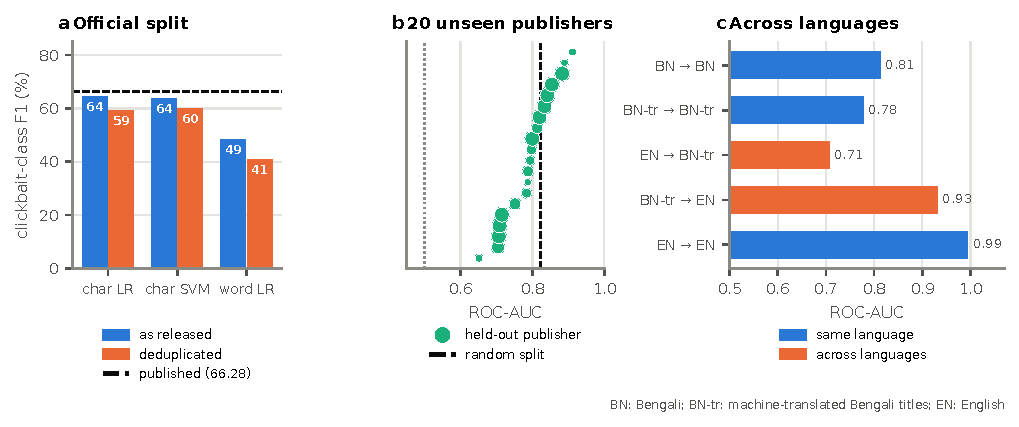
\includegraphics[width=\linewidth]{fig_bengali}
\caption{Bengali clickbait. (a)~Clickbait-class F1 on the official BanglaBait split, as released and after removing near-duplicates, against the published value for character LR \citep{mahtab2023banglabait}. (b)~ROC-AUC on each held-out publisher (dot size: number of articles) against the random-split value. (c)~Translate-test: training and test corpora in Bengali (BN), machine-translated Bengali titles (BN-tr) or English clickbait headlines (EN).}\label{fig:bengali}
\end{figure}


\section{Discussion}\label{sec:discussion}

\paragraph{What the benchmarks measure}
Every corpus in our suite can be told apart from every other with high accuracy (proxy $\mathcal{A}$-distance \PADmin--\PADmax{} on a scale whose maximum is 2). On the article corpora a model of surface statistics recovers nearly all of the in-domain signal, and on average more than half of it. The article and tweet corpora reach most of their final AUC with 64 training examples, and the heaviest feature weights point to outlet signatures and to the time window in which the fake class was collected (Section~\ref{sec:shortcuts}). To a large extent, then, in-domain scores measure how well a model recognises the \emph{collection process} behind each class. \citet{verma2026audit} reached the same conclusion for ISOT alone. Our matrix shows that it holds across units and constructs, and that what is lost on a new corpus is mostly ranking, with calibration a smaller part.

\paragraph{What to do about it}
The decomposition separates a cheap problem from a hard one. The operating-point part is cheap. Rate transfer needs no target labels and one line of code, and it recovered \RecRank{} of that loss for \textsc{tfidf-lr} and between \RecRankMin{} and \RecRankMax{} across detectors, while the textbook label-shift correction made things worse for all of them. Someone deploying a detector on a new feed should therefore fix the \emph{share} of items they flag, not a score threshold. If the base rate of the feed is expected to differ from the training data, labelling a small sample to estimate it is the better investment, since neither label-free prior estimator we tested could do it (Section~\ref{sec:op}).

The ranking part is hard. Source diversity helped: pooled training reached \LocoPooled{} held-out AUC against \LocoMeanSingle{} for a single source. But label-free invariance methods made ranking worse, and the pooled model is still far below the in-domain ceiling of \LocoCeiling{}. Invariance to corpus identity is not enough when the label itself is tied to how each corpus was put together. Better ranking will need better data, in particular corpora whose real and fake items come from the same outlets and time windows, or evidence-based detectors that do not lean on style \citep{pelrine2023gpt4,thibault2025guide}. Multi-domain architectures \citep{nan2021mdfend,zhu2022endef} should be evaluated on held-out corpora with this entanglement in mind.

\paragraph{Style as construct and as shortcut}
The Bengali results add a distinction that the English matrix alone would not show. Clickbait detection held up on unseen publishers and partly across a change of language, while veracity detection did not survive a change of corpus. A plausible explanation is that a style-sensitive model transfers when style \emph{is} the construct, as with clickbait headlines, and fails when style is only correlated with the label inside one collection, as with fake news. With a single Bengali corpus and labels made in different ways, we offer this as a hypothesis for benchmark designers, not a settled result: they should say which kind of cue their labels license.

\begin{protocol}
For any claim that a misinformation detector generalises:
(1)~\emph{verify label direction} with signature probes, and treat a same-task AUC below 0.5 as a data error until shown otherwise;
(2)~\emph{deduplicate} within and across corpora with near-duplicate matching, and drop label-conflicting groups;
(3)~report at least one \emph{same-task cross-corpus} result, with a ranking metric (ROC-AUC or AP) next to F1;
(4)~report the \emph{decomposition}: F1 at the default, prior-matched and (cross-fitted) oracle thresholds;
(5)~run three cheap \emph{shortcut probes}: a surface-statistics model, a group-identity baseline where metadata exist, and a 64-example learning-curve point;
(6)~report a \emph{permutation control}, several seeds, and intervals that resample corpora when averaging over a matrix;
(7)~deploy with a \emph{rate-based} operating point unless target labels are available, and estimate the target base rate from a labelled sample if it is expected to change.
\end{protocol}

\subsection{Limitations and threats to validity}\label{sec:limits}
\emph{Models.} Six of our detectors are linear or tree-based on sparse, static-embedding and frozen RoBERTa features. The seventh fine-tunes only the upper four layers of RoBERTa-base, on 800 training items per corpus and three seeds, because the study ran on a two-core CPU; full fine-tuning on the complete splits might do better in-domain, though prior work found that it does not reliably help across corpora \citep{verma2026audit,delloglio2026comparison}. We did not prompt large language models, which earlier studies found more robust across corpora \citep{pelrine2023gpt4,delloglio2026comparison}. The decomposition applies unchanged to any detector that outputs a score, and testing it on those families is the most direct extension.
\emph{Corpora.} Labels differ in kind (claims, stories, outlets), which is why we lean on same-task pairs. FakeNewsNet is used through its public titles only. NELA-GT and BanFakeNews could not be obtained in our environment, so the Bengali analysis uses one Bengali corpus and a translate-test rather than a second native corpus. PHEME labels rumours, not falsehood, and serves only as an additional unit. The article corpora enter as cleaned working copies (Section~\ref{sec:data}). Deduplication thresholds (Jaccard $\geq$ 0.8) trade recall for precision, and looser thresholds would remove more items.
\emph{Statistics.} Twitter15/16 and PolitiFact test sets are small, so their cells have wide intervals (Table~\ref{tab:pairs}). We report pooled seed-bootstrap intervals per cell, resample corpora for matrix-level quantities, and avoid conclusions from single small cells. Seven corpora are still few, and the corpus-level intervals are correspondingly wide.
\emph{Operating points.} Rate transfer worked here partly because the base rates of our corpora are similar. The prior-shift experiment shows how it degrades when they are not; that experiment resamples existing test sets and does not reproduce every way a real feed can change.
\emph{Scope.} Our results concern text-only detection. Propagation-based detectors face related spurious-correlation problems on Twitter15/16 and PHEME \citep{wu2022spurious,mu2023time,pelrine2021simple}, which we did not re-evaluate.
\emph{Ethics.} We use only released text of public posts, with no user identifiers and no re-collection. Tweet content remains subject to the platform's terms, so we release code, per-cell results and saved scores but no post text.

\section{Conclusion}\label{sec:conclusion}
Misinformation detectors that look near-perfect in-domain lose much of their value on a new corpus, though not all of it, and not for a single reason. Across ten audited corpora and seven detectors, \RankShareAll{} of the macro-F1 they lose is a ranking deficit that only better data or representations can address. The remaining \OpShareAll{} is a misplaced operating point, and most of it can be repaired without a single target label by transferring the share of items the detector flags rather than trusting its scores or a label-shift correction. That repair is exact when target scores are an order-preserving distortion of source scores and the base rate is unchanged, and it weakens as the base rate moves. A zero-shot language model shows the opposite balance, ranking unseen corpora better than any transferred detector while losing mostly its operating point, which the same rule repairs; published domain-generalisation methods, by contrast, do not improve on simply pooling the training corpora. Much of what in-domain benchmarks reward is the collection process behind each class: outlet signatures, attribution style, time windows. Where style is the construct itself, as with clickbait, detection travels across publishers and in part across languages; where it is a by-product of how a corpus was assembled, as with veracity, it does not. Papers that claim generalisation should report transfer, ranking metrics and the decomposition next to in-domain accuracy, and the protocol and code released with this paper make that cheap to do.


\section*{CRediT authorship contribution statement}
\textbf{Dewan Fahad Chowdhury:} Conceptualization (equal), Methodology (equal), Software (lead), Formal analysis (lead), Investigation (equal), Data curation (equal), Visualization (lead), Writing -- original draft (lead), Writing -- review \& editing (equal). \textbf{Md.\ Rejaul Korim Sadi:} Conceptualization (equal), Methodology (equal), Validation (lead), Investigation (equal), Data curation (equal), Writing -- review \& editing (equal), Project administration (lead).

\section*{Declaration of competing interest}
The authors declare that they have no known competing financial interests or personal relationships that could have appeared to influence the work reported in this paper.

\section*{Funding}
This research did not receive any specific grant from funding agencies in the public, commercial, or not-for-profit sectors.

\section*{Data and code availability}
All corpora are publicly available from their original releases (Section~\ref{sec:data} and the repository's \texttt{DATA.md}); none is redistributed. Code, fixed seeds, per-cell results, saved predictions, logs and a one-command reproduction script are released under the MIT licence at \url{https://github.com/<account>/fn-transfer-audit} (archived release DOI to be added on acceptance).

\section*{Declaration of generative AI and AI-assisted technologies in the manuscript preparation process}
The research questions, study design, choice of corpora and interpretation of the results are the authors' own. During the preparation of this work the authors used Claude (Anthropic) in order to help implement and check the analysis code, organise the manuscript, typeset it in LaTeX and edit its language. After using this tool, the authors reviewed, verified and edited all code, results and text as needed and take full responsibility for the content of the published article.

\bibliographystyle{elsarticle-harv}
\bibliography{refs}

\appendix
\section{Proof of Proposition~\ref{prop:rate}}\label{app:proof}
Write $M^A(u)=\pi_A F^A_1(u)+(1-\pi_A)F^A_0(u)$ for the distribution function of source scores and $M^B$ for that of target scores, and assume $M^A$ is continuous and strictly increasing around $\tau_0$, so that quantiles are unique. The source model flags $q_A=1-M^A(\tau_0)$ of the source items.

\emph{Rate transfer under (i) and (ii).} By (i) and (ii), $M^B(g(u))=\pi_A F^B_1(g(u))+(1-\pi_A)F^B_0(g(u))=M^A(u)$ for every $u$. The threshold that flags the top $q_A$ share of target items is the $t$ with $M^B(t)=1-q_A=M^A(\tau_0)$, that is, $t=g(\tau_0)$. Its true-positive rate on $B$ is $1-F^B_1(g(\tau_0))=1-F^A_1(\tau_0)$, the source true-positive rate at $\tau_0$, and the same argument holds for the false-positive rate. With equal priors, equal error rates give the same expected confusion matrix, and hence the same population macro-F1 and balanced accuracy. The fixed threshold $\tau_0$ has true-positive rate $1-F^A_1(g^{-1}(\tau_0))$ on $B$, which equals the source rate for every pair of class distributions only if $g^{-1}(\tau_0)=\tau_0$. EM is also misled under (i): it assumes $F^B_y=F^A_y$, so a monotone distortion of the scores is read as a change of class balance.

\emph{Pure label shift.} If $g$ is the identity and $\pi_B\neq\pi_A$, then $p_B(x\mid y)=p_A(x\mid y)$, calibrated source posteriors are related to target posteriors by Bayes' rule with the two priors, and the EM fixed point of \citet{saerens2002adjusting} is the true $\pi_B$ in the population limit. The share of target items above $\tau_0$ is $\pi_B\mathrm{TPR}_A+(1-\pi_B)\mathrm{FPR}_A$, which differs from $q_A$ whenever $\mathrm{TPR}_A\neq\mathrm{FPR}_A$. Rate transfer therefore moves the threshold away from $\tau_0$ even though the class-conditional score distributions have not changed, so it no longer reproduces the source error rates, and in general it does not coincide with the Bayes threshold for $\pi_B$ either. $\square$

\section{Implementation details and compute}\label{app:impl}
\paragraph{Hyperparameters}
Logistic regression and linear SVM: $C\in\{0.25,1,4\}$ (SVM: $C/4$), liblinear, selected by validation ROC-AUC; TF-IDF word 1--2-grams, \texttt{min\_df}=2, 100{,}000 features, sublinear term frequency, texts truncated to 20{,}000 characters. NB-SVM: binary 1--2-grams, add-one smoothed log-count ratios. GloVe: 100-d \texttt{glove-wiki-gigaword}, mean of in-vocabulary tokens. Style model: histogram gradient boosting with 100 or 300 iterations, learning rate 0.1. Frozen RoBERTa: mean of last-layer piece states, standardised, logistic regression with $C\in\{0.025,0.1,0.4\}$. Fine-tuned RoBERTa: lower eight layers frozen and cached, upper four layers and a linear head trained with AdamW for three epochs (details in the Supplementary Material). Platt scaling on the validation split for every model. Bengali: character 3--5-grams (\texttt{char\_wb}), 200{,}000 features.
\paragraph{Deduplication}
MinHash with 128 permutations (seed 1) and LSH at Jaccard 0.8; word 3-gram shingles over the first 400 words for articles, character 5-grams otherwise; text normalised with NFKC, lower-casing, URL and punctuation removal.
\paragraph{Compute}
All experiments ran on a 2-core CPU with 8\,GB RAM and no GPU. The full pipeline (\texttt{run\_all.sh}) takes about ten to twelve hours, plus roughly four hours for caching and fine-tuning the transformer. Software: Python 3.13, scikit-learn 1.9.1, spaCy 3.8, PyTorch 2 (CPU), datasketch, statsmodels.

\section{Reproducibility checklist}\label{app:checklist}
\begin{itemize}
\item Data: public sources, licences and expected layout in \texttt{DATA.md}; label harmonisation and its verification in \texttt{src/label\_probe.py}; deduplication counts in \texttt{results/dedup\_report.json}.
\item Splits and seeds: five seeds (0--4; three for the fine-tuned transformer) fix splits, subsampling and model initialisation; vectorisers and calibrators are fitted on source training and validation data only.
\item Every number in this paper is written by \texttt{src/paper\_numbers.py} from the files in \texttt{results/}; no number is typed by hand.
\item Saved per-item scores for every (model, source, target, seed) cell allow any metric or threshold rule to be recomputed without retraining.
\item Sanity controls: permutation regime (AUC $\approx$ 0.5) and size-matched regime are part of the main grid.
\item The Supplementary Material contains the full matrices for every model, per-cell decompositions and operating points, learning curves, the vocabulary ablation, per-publisher Bengali results and the deduplication report.
\end{itemize}

\end{document}
